\documentclass[11pt]{amsart}
\usepackage[T1]{fontenc}
\usepackage{lmodern}
\usepackage{mathtools,amssymb,graphicx,booktabs,enumitem,array}
\usepackage[hidelinks]{hyperref}
\hypersetup{
  pdftitle={The 3-Adic Dicyclic Companion, Exact Level 3P5 and Level (3) Congruence on Nauru, and the Real-Quadratic Lame Shimura Curve Atlas},
  pdfauthor={Ergentics},
  pdfkeywords={Nauru graph, dicyclic group Dic6, Ramanujan graph, Ihara-Hashimoto zeta function, 2-adic Mumford curve, 3-adic Mumford curve, Lame quaternion algebra, Fricke-Vogt moduli, congruence Shimura curve, Eichler order, Riehm theorem, scramble number, metric gonality, Poitou-Odlyzko explicit formula}
}
\pdfinfo{/Producer () /Creator ()}
\usepackage{microtype}
\numberwithin{equation}{section}
\theoremstyle{plain}
\newtheorem{theorem}{Theorem}[section]
\newtheorem{proposition}[theorem]{Proposition}
\newtheorem{lemma}[theorem]{Lemma}
\newtheorem{corollary}[theorem]{Corollary}
\theoremstyle{definition}\newtheorem{definition}[theorem]{Definition}
\theoremstyle{remark}\newtheorem{remark}[theorem]{Remark}
\newcommand{\Q}{\mathbb{Q}}
\newcommand{\R}{\mathbb{R}}
\newcommand{\C}{\mathbb{C}}
\newcommand{\Z}{\mathbb{Z}}
\newcommand{\F}{\mathbb{F}}
\newcommand{\calO}{\mathcal{O}}
\newcommand{\calE}{\mathcal{E}}
\newcommand{\calC}{\mathcal{C}}
\newcommand{\calS}{\mathcal{S}}
\newcommand{\frP}{\mathfrak{P}}
\newcommand{\frp}{\mathfrak{p}}
\newcommand{\frq}{\mathfrak{q}}
\newcommand{\PGL}{\mathrm{PGL}}
\newcommand{\PSL}{\mathrm{PSL}}
\newcommand{\SL}{\mathrm{SL}}
\newcommand{\GL}{\mathrm{GL}}
\newcommand{\Aut}{\mathrm{Aut}}
\newcommand{\Cay}{\mathrm{Cay}}
\newcommand{\GP}{\mathrm{GP}}
\newcommand{\Dic}{\mathrm{Dic}}
\newcommand{\Stab}{\mathrm{Stab}}
\newcommand{\Ad}{\mathrm{Ad}}
\newcommand{\Ram}{\mathrm{Ram}}
\newcommand{\nrd}{\operatorname{nrd}}
\newcommand{\trd}{\operatorname{trd}}
\newcommand{\gon}{\operatorname{gon}}
\newcommand{\dgon}{\operatorname{dgon}}
\newcommand{\sn}{\operatorname{sn}}
\newcommand{\ctag}[1]{\textup{\textsf{\scriptsize[#1]}}}
\emergencystretch=4em\hbadness=10000
\raggedbottom

\title[3-Adic \texorpdfstring{$\Dic_6$}{Dic6}, Nauru Congruence \& Real-Quadratic Atlas]{The 3-Adic Dicyclic Companion, Exact Level \texorpdfstring{$3\frP_5$}{3P5} and Level \texorpdfstring{$(3)$}{(3)} Congruence on Nauru, and the Real-Quadratic Lam\'e Shimura Curve Atlas}
\author{Ergentics}
\date{November 2026}
\subjclass[2020]{Primary 11G18, 14G22, 05C50; Secondary 05C57, 11R52, 20E08}
\keywords{Nauru graph, dicyclic group $\Dic_6$, Ramanujan graph, Ihara--Hashimoto zeta function, $p$-adic Mumford curve, Lam\'e quaternion algebra, Fricke--Vogt moduli, congruence Shimura curve, Eichler order, Riehm's theorem, scramble number, metric gonality, Poitou--Odlyzko explicit formula}

\begin{document}
\begin{abstract}
We resolve the higher-degree arithmetic, tropical-metric, $3$-adic moduli, and explicit-formula frontiers opened by \emph{Prime Cadences} (Paper~\#01 \cite{ergentics2026pc}) and its companion study \emph{Uniform Triadic Wreath Products, the Nauru Graph, and Dual-Prime $D=6$ Arithmeticity} (Paper~\#08 / \texttt{PC-II} \cite{ergentics2026pc2}), backed by four independent zero-shared-data continuous-integration verification planes (pure Python, zero-crate Rust, freestanding zero-heap hardware-\texttt{FENV} C++20, and live kernel-compiled zero-Mathlib Lean~4.36.0).
First (\textbf{Pillar~I}), we prove the universal algebraic twin duality $\tau((bt)a) = 3 - x$ on the $2$-adic Lam\'e quaternion family $B(x) = (-3, -x(3-x)/F)$ exchanging the two Nauru graph-automorphism surjections $\rho_6 \leftrightarrow \rho_{12}$, separate the genuine level-$3\frP_5$ congruence Shimura curve $(B_5, \frac{5}{2}, \rho_6) \cong (B_5, \frac{1}{2}, \rho_{12})$ ($|\Ad_{15}| = |\mathrm{joint}| = 3600 = 144\times 25$, unique normal Sylow-$5$ $U_5$ killed since $\gcd(25,144)=1$) sharply from both non-congruence $V_4$-covers ($B_3(\frac{3}{2}) \to X^6(\Gamma(3)) \leftrightarrow K_{3,3}$ at level~$3$ vs.\ $(B_5, \frac{1}{2}, \rho_6) \to X^{10}(\Gamma(3\frP_5))/V_4 \leftrightarrow K_{3,3}$ only at level~$3\frP_5$), reconcile all historical \texttt{PC-II} errata (\texttt{NEG-M19}, \texttt{NEG-M23}, \texttt{NEG-M24}: $\pi_Y(18)=28{,}560$, $\pi_Y(22)=380{,}664$, $|[G,G]|/|G^{\mathrm{ab}}|=6/24$), and prove unconditional metric gonality $\sn(Y) = \dgon(Y) = \gon(\Gamma_{\mathrm{eq}}(Y)) = 6 \le \gon(\Gamma(Y)) \le \gon(\calC_Y)$ via $132/132$ continuous Dhar cells.
Second (\textbf{Pillar~II}), we classify all $6$ primitive real-quadratic Lam\'e Nauru moduli across $4$ totally real fields---all with $\Ram_{\mathrm{fin}}(B(x)) = \varnothing$---resolving every field's exact congruence status (\texttt{NEG-M25}): non-congruence $\Z/3\Z$-cover of the Cube Shimura curve $X^{17}(\Gamma(v^2)) \leftrightarrow Q_3$ over $\Q(\sqrt{17})$; strictly non-congruence Eichler-$\frq_7$ cover of $X^1(\frq_7) \leftrightarrow \Theta_3$ over $\Q(\sqrt{2})$ ($\calE(\frq_7)$, $T_8\text{-}\det = 49\cdot 8^4$, $|\ker^1|=12$ with non-isomorphic Galois kernels $C_6\times C_2$ vs.\ $A_4$, obstructed by $4\nmid 1$); strictly non-congruence over $\Q(\sqrt{3})$ via the Eichler-$\frp_3$ $2$-part obstruction ($|\Ad_3^1|=243, |\Ad_3^+|=486, |\Ad_3|=972$); and a \textbf{second genuine congruence Shimura curve of exact level $(3) = \frp_3\frp_3'$ for both $\rho_6$ and $\rho_{12}$ over $\Q(\sqrt{7})$} ($|\Ad_{(3)}| = |\mathrm{joint}| = 576$, $|\ker| = 1$, $144/144$), complemented by the complete census of all $4$ irreducible totally real cubic moduli ($d_F \in \{148, 316\}$).
Third (\textbf{Pillar~III}), we solve the rational $3$-adic $\Dic_6$ moduli problem on $T_4(\Q_3)$: classifying all $18$ connected $4$-regular $\Dic_6$ Cayley graphs ($12$ Ramanujan $Z$ with exact $\pi_Z(4..16)$, $6$ boundary), collapsing metric gonality $\sn(Z) = \dgon(Z) = \gon(\Gamma_{\mathrm{eq}}(Z)) = 8 \le \gon(\Gamma(Z)) \le \gon(\calC_Z)$ via the optimal $4$-path scramble $\calS_4$ ($h=e=8$), exhaustive Dhar ($0/98{,}280$ at deg~$6$, $0/475{,}020$ at deg~$7$), and $168/168$ continuous Dhar cells on both $D_8 = \langle x^3\rangle + \langle x^3\rangle y$ and \texttt{PC-II}'s $D_{\Dic_6}$, classifying all $5/10$ rational arithmetic Fricke--Vogt moduli $B_Z(u,v)$ via $4\mid mn$, proving universal rational non-congruence ($0/80$ realizations across both adjoint and diagonal-$\pm 1$ CRT true left-multiplication $\Gamma(M)$, closed at all levels via Riehm's theorem and Burnside's Basis Theorem), reconciling Hurwitz $B_2(4,4)$ level-$8$ left-multiplication ($|L_8/\{\pm 1\}|=64$ already attains $|\ker^1|=3$ across $16/16$, matching \texttt{PC-II} Theorem~7.2) with level-$16$ adjoint ($\Ad_{16}=1024$, \texttt{NEG-M26}), and pairing the $19$-curve ($9$ torsion-free) genus-$25$ Borel Shimura census with \texttt{PC-II} Theorem~7.3's $0/19$ Manin $T_3$ exclusion.
Finally, we deliver a hardware-\texttt{FENV} strict-Bochner-positivity Poitou--Odlyzko audit certifying $18.6606783717 > 18.6470485626$ while rejecting sign-changing facade kernels and preserving the degree-$8$ $(8,1,1,E)$ gap ($12.593730$ at $b=3.0$, exact continuous peak $12.595576$ at $b^*\approx 3.0399 < 13.142385$, \texttt{NEG-M27}).
\end{abstract}
\maketitle

\section{Introduction and Summary of Main Results}\label{sec:intro}
The interplay between finite symmetric Ramanujan graphs, Ihara--Hashimoto--Bass graph zeta functions \cite{ihara1966,hashimoto1989,bass1992,starkterras1996,terras2011,lps1988}, $p$-adic Mumford uniformization \cite{mumford1972,drinfeld1976,gvdp1980,serre1980,kato2005,ck2005}, quaternion Shimura curves \cite{eichler1955,shimura1967,vigneras1980,voight2021}, and tropical Brill--Noether specialization \cite{bakernorine2007,baker2008,bpr2013,dhar1990,hjjs2022} has driven the Morpheus research program from Paper~\#01 (\emph{Prime Cadences} \cite{ergentics2026pc}, analyzing the $24$-vertex cubic neo-Riemannian Tonnetz graph $X$ \cite{tymoczko2011,cohn2012}) through Paper~\#08 / \texttt{PC-II} (\cite{ergentics2026pc2}, passing to its $144$-automorphism bipartite Ramanujan sibling, the Nauru graph $Y = \GP(12, 5)$, and its $3$-adic Hurwitz $B_2$ companion $Z = \Cay(\Dic_6, \{x, x^{-1}, y, y^3\})$).

While \texttt{PC-II} (\texttt{v0.7.1}) resolved the $D=6$ dual-prime arithmetic mirror over $\Q$, four major mathematical frontiers remained open or required complete multi-field and continuous-metric resolution:
\begin{enumerate}[label=(\arabic*),nosep]
\item establishing universal algebraic twin duality $\tau((bt)a) = 3 - x$ on the Lam\'e family $B(x) = (-3, -x(3-x)/F)$, separating the congruence levels of all rational Nauru covers across both surjections $\rho_6, \rho_{12}$, and upgrading divisorial gonality $\dgon(Y) = 6$ to an \emph{unconditional continuous metric} lower bound $\sn(Y) = \gon(\Gamma_{\mathrm{eq}}(Y)) = 6 \le \gon(\Gamma(Y)) \le \gon(\calC_Y)$;
\item classifying the complete real-quadratic and totally real cubic Lam\'e Nauru moduli, proving $\Ram_{\mathrm{fin}}(B(x)) = \varnothing$ uniformly across all $6$ real-quadratic curves, constructing explicit ring-closed maximal and Eichler orders for all $4$ real-quadratic fields, and determining their exact congruence status (culminating in a second genuine congruence Shimura curve over $\Q(\sqrt{7})$ at exact level $(3)=\frp_3\frp_3'$);
\item resolving the full rational $2$-parameter Fricke--Vogt moduli surface $B_Z(u,v)$ for the $3$-adic dicyclic graph $Z$ on the $4$-regular Bruhat--Tits tree $T_4(\Q_3)$, proving exact metric gonality collapse $\sn(Z) = \dgon(Z) = \gon(\Gamma_{\mathrm{eq}}(Z)) = 8 \le \gon(\calC_Z)$ via an optimal $4$-path scramble $\calS_4$, proving universal $0/80$ rational non-congruence at all levels via diagonal-$\pm 1$ CRT true left-multiplication $\Gamma(M)$ and Riehm's theorem \cite{riehm1970}, and reconciling adjoint vs.\ left-multiplication level behavior on Hurwitz $B_2(4,4)$ with \texttt{PC-II} Theorem~7.2;
\item auditing strict Bochner positivity in the Poitou--Odlyzko explicit-formula discriminant lower bounds \cite{poitou1977,odlyzko1990} used in Paper~\#01 Theorem~7.21 via hardware-rounded IEEE-754 interval arithmetic \cite{moore1966}.
\end{enumerate}

\begin{remark}[Attribution, Reconciliation with \texttt{PC-II}, and Four-Plane CI Verification]\label{rem:attribution}
Following Morpheus governance (\path{AGENTS.md}, \path{METHODOLOGY.md}), attribution tags record \ctag{lit.} classical literature, \ctag{E} research direction and clean-room monograph derivations by Ergentics, \ctag{G4N} independent first-principles cross-verification, reconciliation, and continuous-testing formalization by Gemini~4~Neon, and \ctag{X} zero-shared-data multi-plane cross-verification. Earlier \texttt{PC-II} \texttt{v0.5.0}--\texttt{v0.7.0} discrepancies surfaced during independent clean-room cross-auditing ($B_5(\frac{5}{2})$ level $3\frP_5$ congruence \texttt{NEG-M23}, $\langle T,P,L,R\rangle$ commutator $6/24$ \texttt{NEG-M19}, and $\pi_Y(18)=28{,}560, \pi_Y(22)=380{,}664$ \texttt{NEG-M24}) have been repaired in \texttt{PC-II v0.7.1} \cite{ergentics2026pc2} and are independently re-certified here. Every theorem below is verified live in continuous integration across four independent zero-shared-data Code-Model planes inside \path{papers/triadic_3adic_frontier/}:
(1)~pure Python stdlib (\path{code/triadic_3adic_verify.py}, $8/8$ gates \texttt{F1}--\texttt{F8} + \texttt{--check-only} CI parity against SHA-256-manifested \path{data/triadic_3adic_calibration.json});
(2)~zero-crate Rust (\path{rust/src/lib.rs}, $6/6$ integration tests and core suites incl.\ exhaustive deg-$6$/$7$ Dhar and all $80/80$ CRT left-mult);
(3)~freestanding zero-heap hardware-\texttt{FENV} C++20 (\path{cpp/fenv_oracle.cpp}, $6/6$ gates compiled with \texttt{-O2 -std=c++20 -frounding-math -Wall -Wextra -Werror}); and
(4)~live kernel-compiled zero-Mathlib Lean~4.36.0 \cite{mouraullrich2021} (\path{lean/Triadic3AdicFrontier/}, $20/20$ theorems compiled under \texttt{-DwarningAsError=true -DautoImplicit=false}, $0$ \texttt{sorryAx}, $0$ \texttt{Lean.ofReduceBool}).
\end{remark}

\subsection{Notation Hygiene}\label{sec:notation}
We write $\Z_p$ for the $p$-adic integers and $\Q_p$ for its fraction field; finite cyclic groups of order $m$ are written $\Z/m\Z$ or $C_m$, and $V_4 = \Z/2\Z \times \Z/2\Z$. The Nauru graph is $Y = \GP(12,5)$ ($V=24, E=36, g=b_1(Y)=13$, girth~$6$), and the $4$-regular dicyclic Cayley graph is $Z = \Cay(\Dic_6, \{x,x^{-1},y,y^3\})$ ($V=24, E=48, g=b_1(Z)=25$, girth~$4$). For a finite graph $G$, $\pi_G(m)$ counts equivalence classes (up to cyclic shift) of primitive non-backtracking tailless closed walks of length $m$, with Hashimoto trace $N_m(G) = \operatorname{tr}(T_G^m) = \sum_{d\mid m} d\,\pi_G(d)$. For a smooth projective curve $\calC$ over a complete non-Archimedean field with minimal Berkovich skeleton $\Gamma(G)$, $\gon(\calC)$, $\gon(\Gamma(G))$, $\gon(\Gamma_{\mathrm{eq}}(G))$, $\dgon(G)$, and $\sn(G)$ denote algebraic gonality, metric gonality, equilateral metric gonality, discrete divisorial gonality, and scramble number. For a quaternion algebra $B = (\alpha,\beta/F)$, $\tau(\gamma) = \trd(\gamma)^2/\nrd(\gamma)$ is the projective trace invariant and $\Ram_{\mathrm{fin}}(B)$ is the finite ramification set. For rational Shimura curves, $X^D(\Gamma(M))$ denotes indefinite quaternion discriminant $D$ and level $M$; over $F = \Q(\sqrt{17})$ where $\Ram_{\mathrm{fin}}(B) = \varnothing$, $X^{17}(\Gamma(v^2))$ labels field discriminant $D_F=17$, quaternion discriminant $(1)$, and level $v^2$.

\begin{table}[htbp]
\centering
\caption{Summary of Pillars~I--III, the Poitou--Odlyzko strict-positivity audit, and live four-plane CI certificates.}
\label{tab:summary}
\footnotesize
\setlength{\tabcolsep}{4pt}
\resizebox{\textwidth}{!}{\begin{tabular}{@{}l>{\raggedright\arraybackslash}p{2.7cm}>{\raggedright\arraybackslash}p{6.6cm}l@{}}
\toprule
\textbf{Track} & \textbf{Principal Object} & \textbf{Headline Resolution} & \textbf{CI Planes} \\
\midrule
Pillar~I & Rational $2$-adic Nauru $Y$ & Twin duality $\tau((bt)a)=3-x$; level $3\frP_5$ cong.\ $(B_5,\tfrac{5}{2},\rho_6)$ ($3600$, $\gcd(25,144)=1$); $B_3(\tfrac{3}{2})\to X^6(\Gamma(3))$ vs.\ $B_5(\tfrac{1}{2},\rho_6)\to X^{10}(\Gamma(3\frP_5))/V_4$; $\sn=\dgon=\gon_{\mathrm{eq}}=6$ ($132/132$ cells) & Py, Rust, C++, Lean \\
Pillar~II & Real-quad.\ \& cubic Lam\'e atlas & $6$ real-quad.\ moduli ($4$ fields, $\Ram_{\mathrm{fin}}=\varnothing$): $\Q(\sqrt{17})$ ($Q_3$, $|\ker|=3$), $\Q(\sqrt{2})$ ($\calE(\frq_7)\to\Theta_3$, $C_6{\times}C_2/A_4$), $\Q(\sqrt{3})$ ($\calE(\frp_3)$, $2$-part $1<4$), $\Q(\sqrt{7})$ \textbf{cong.\ level $(3)$} ($576$, $144/144$ both $\rho_6,\rho_{12}$); $4$ cubic moduli ($d_F\in\{148,316\}$) & Py, Rust, Lean \\
Pillar~III & $3$-adic $\Dic_6$ on $T_4(\Q_3)$ & $18$ Cayley ($12$ Ram.\ $Z$, $6$ bnd.); $\pi_Z(4..16)$; $\sn=\dgon=\gon_{\mathrm{eq}}=8$ ($\calS_4$, $D_8$, $0/475{,}020$ deg~$7$); $5/10$ Fricke--Vogt ($4\mid mn$); $0/80$ cong.\ (CRT $\Gamma(M)$ + Riehm mod~$8$); Hurwitz $L_8/\{\pm 1\}=64$ vs.\ $\Ad_{16}=1024\to K_{4,4}$; $19$ ($9$ TF) genus-$25$ ($0/19$ by \texttt{PC-II} Thm~7.3) & Py, Rust, C++, Lean \\
Audit & Poitou--Odlyzko \texttt{FENV} gate & Strict Bochner pos.\ $18.6606783717 > 18.6470485626$ (gap $\ge +0.013629809157$); $f_{\mathrm{bad}}(\pm 1)=-0.60$ rejected; $(8,1,1,E)$ gap preserved ($12.593730$ at $b=3.0$, peak $12.595576$ at $b^*=3.0399 < 13.142385$) & Py, Rust, C++ \texttt{FENV} \\
\bottomrule
\end{tabular}}
\end{table}

\section{Pillar I: Rational 2-Adic Nauru Congruence, Twin Duality, and Metric Gonality}\label{sec:pillar1}
Define the Nauru graph $Y = \GP(12,5)$ on $V(Y) = \{0,\dots,23\}$ with outer $12$-cycle $(i, (i+1)\bmod 12)$, radial spokes $(i, 12+i)$, and inner star edges $(12+i, 12+(i+5)\bmod 12)$ for $i\in\Z/12\Z$. Exact backtracking confirms $|\Aut(Y)| = 144$, with vertex stabilizer $\Stab_0 = \langle a_Y, b_Y\rangle \cong S_3$ ($\operatorname{ord}(a_Y)=3$, $\operatorname{ord}(b_Y)=2$, $b_Y$ fixing $\{0,12\}$ pointwise) and edge stabilizer $\Stab_{\{0,12\}} \cong V_4$. Inside $\Stab_{\{0,12\}}$ lie exactly two edge-inverting involutions exchanging $0 \leftrightarrow 12$, namely $t_0$ and $t_1 = b_Y t_0 = t_0 b_Y$, sharply separated by
\begin{equation}\label{eq:rho6_rho12}
\operatorname{ord}(t_0 a_Y) = 6, \qquad \operatorname{ord}(t_1 a_Y) = 12.
\end{equation}
Thus every $2$-adic arithmetic amalgam $\Delta = \langle a, b, t\rangle$ acting vertex- and edge-transitively on $T_3(\Q_2)$ with vertex stabilizer $S_3 = \langle a, b\rangle$ and edge-inverting involution $t$ (commuting with $b$ in $PB^\times$) admits exactly two conjugacy classes of surjections onto $\Aut(Y)$: $\rho_6$ ($t \mapsto t_0$) and $\rho_{12}$ ($t \mapsto t_1 = b_Y t_0$).

\subsection{Universal Algebraic Twin Duality on the Lam\'e Family \texorpdfstring{$B(x)$}{B(x)}}\label{sec:twin_duality}
\begin{proposition}[Universal Algebraic Twin Duality $\tau((bt)a) = 3 - x$]\label{prop:twin_duality}
\ctag{E; G4N, X, Lean~4}\ In the universal $2$-adic Lam\'e quaternion algebra $B(x) = (-3, -x(3-x)/F)$ ($A=-3, B=-x(3-x)$, $i^2=A, j^2=B, ij=k=-ji$) over any field $F$ of characteristic $0$, with vertex stabilizer generators $a=(1+i)/2$ ($a^3=-1$) and $b=j$ ($bab^{-1}=\bar a$), and any pure-imaginary edge-inverting involution $t = ui + vk$ ($u,v\in F$, $btb^{-1}=-t$) normalized so that $\tau(ta)=x$, one has the exact identities
\begin{equation}\label{eq:twin_duality}
\tau(ta) = \frac{3u^2}{u^2 - Bv^2} = x, \qquad \tau((bt)a) = \frac{-3Bv^2}{u^2 - Bv^2} = 3 - x.
\end{equation}
In particular, $t = xi + k$ ($\nrd(t)=9x$) satisfies $\tau(ta)=x$ and $\tau((bt)a)=3-x$, so replacing $t \mapsto bt$ induces canonical isomorphisms of marked $2$-adic Mumford curves $(B(x),\rho_6) \cong (B(3-x),\rho_{12})$ and $(B(x),\rho_{12}) \cong (B(3-x),\rho_6)$.
\end{proposition}
\begin{proof}
Direct multiplication yields $ta = (ui+vk)(1+i)/2 = (-3u + ui + 3vj + vk)/2$, so $\trd(ta)=-3u$ and $\nrd(ta) = 3(u^2 - Bv^2)$, giving $\tau(ta) = 3u^2/(u^2 - Bv^2)$. Since $ji=-k$ and $jk=-Bi$, we obtain $bt = j(ui+vk) = -Bvi - uk$ and $(bt)a = (3Bv - Bvi - 3uj - uk)/2$, whence $\trd((bt)a) = 3Bv$ and $\nrd((bt)a) = (-B)\cdot 3(u^2 - Bv^2)$. Therefore
\[
\tau((bt)a) = \frac{9B^2 v^2}{-3B(u^2 - Bv^2)} = \frac{-3Bv^2}{u^2 - Bv^2} = 3 - \frac{3u^2}{u^2 - Bv^2} = 3 - \tau(ta) = 3 - x.
\]
Changing the amalgam generator $t \mapsto bt$ composes the map to $\Aut(Y)$ with $t_0 \leftrightarrow b_Y t_0 = t_1$, exchanging $\rho_6 \leftrightarrow \rho_{12}$. The polynomial identity $3u^2 + (-3Bv^2) = 3(u^2-Bv^2)$ and normalized integer form $(-3d)^2 = 9xd(3-x)$ are kernel-checked in Lean~4 (\texttt{thm09}, \texttt{thm10}).
\end{proof}

\subsection{Exact Level \texorpdfstring{$3\frP_5$}{3P5} Congruence and Separation of \texorpdfstring{$V_4$}{V4}-Non-Congruence Covers}\label{sec:rational_nauru}
Over $\Q$, $2$-arithmetic integrality $x \in (0,3)\cap\Z[\frac{1}{2}]$ with $v_2(x)=-1$ restricts to three moduli: the self-twin point $x=\frac{3}{2}$ in $B_3 = (-3,-1/\Q)$ ($D = 2\cdot 3 = 6$) and the twin pair $x \in \{\frac{5}{2},\frac{1}{2}\}$ in $B_5 = (-3,-5/\Q)$ ($D = 2\cdot 5 = 10$). We construct explicit ring-closed maximal orders normalized by $(a,b,t)$ with conjugation denominators $[1,1,2]$:
\begin{enumerate}[label=(\roman*),nosep]
\item $B_3$, $x=\frac{3}{2}$: $\calO_3 = \Z\cdot 1 \oplus \Z\cdot \tfrac{1+i}{2} \oplus \Z\cdot j \oplus \Z\cdot \tfrac{j+k}{2}$ (reduced discriminant $3$), $t_3 = i + k$;
\item $B_5$, $x=\frac{5}{2}$: $\calO_5^- = \Z\cdot 1 \oplus \Z\cdot \tfrac{1+i}{2} \oplus \Z\cdot \tfrac{i-k}{3} \oplus \Z\cdot \tfrac{-3+i-3j-k}{6}$ (reduced discriminant $5$), $t_{5,5/2} = \tfrac{5i+k}{3}$;
\item $B_5$, $x=\frac{1}{2}$: $\calO_5^+ = \Z\cdot 1 \oplus \Z\cdot \tfrac{1+i}{2} \oplus \Z\cdot \tfrac{i+k}{3} \oplus \Z\cdot \tfrac{-3+i+3j+k}{6}$ (reduced discriminant $5$), $t_{5,1/2} = \tfrac{i+k}{3}$.
\end{enumerate}

\begin{theorem}[Exact Level $3\frP_5$ Congruence and Separation of Rational Non-Congruence Covers]\label{thm:rational_cong}
\ctag{E; G4N, X, Lean~4}\ Let $\Delta = \langle a,b,t\rangle \subseteq N_{B^\times}(\calO[\frac{1}{2}])/\Q^\times$.
\begin{enumerate}[label=(\arabic*),nosep]
\item For $(B_5, x=\frac{5}{2}, \rho_6)$---and identically by Proposition~\ref{prop:twin_duality} for its twin $(B_5, x=\frac{1}{2}, \rho_{12})$---the mod-$15$ adjoint action $\Ad_{15} : \Delta \to \Aut(\calO_5^-/15\calO_5^-)$ satisfies $|\Ad_{15}| = |\mathrm{joint}| = 3{,}600 = 144\times 25$, $|\ker| = 1$, and full overlap $144/144$. Inside $\Ad_{15}$, the $25$ elements of order dividing $25$ form a unique normal Sylow-$5$ subgroup $U_5 \trianglelefteq \Ad_{15}$; since $\gcd(25, 144) = 1$ (Lean~4 \texttt{thm13}), $U_5$ maps trivially into $\Aut(Y)$ and $\Ad_{15}/U_5 \cong \Aut(Y)$. As $U_5$ is the $5$-adic pro-unipotent kernel modulo the ramified prime $\frP_5$ ($\frP_5^2 = 5\calO_5^-$), $\calC_Y(B_5, \frac{5}{2}, \rho_6)$ is a \textbf{genuine congruence Shimura curve of exact level $3\frP_5$} on $X^{10}$ (independently matching \texttt{PC-II} Theorem~6.1 \cite{ergentics2026pc2}, \texttt{NEG-M23}).
\item Conversely, the two non-congruence rational families both stabilize with congruence kernel $V_4$ ($|\ker|=4$, overlap $36/144$, quotient dual graph $Y/V_4 \cong K_{3,3}$ with $V=6, E=9$ of uniform multiplicity~$4$, genus~$4$), yet cover \emph{distinct} congruence Shimura curves at different discriminants and levels:
\begin{itemize}[nosep]
\item $(B_3, x=\frac{3}{2})$ ($D=6$, both $\rho_6,\rho_{12}$) already attains overlap $36/144$ ($|\ker|=4$) at \textbf{level $3$} ($|\Ad_3|=36, |\mathrm{joint}|=144$), realizing a non-congruence $V_4$-cover of $X^6(\Gamma(3)) \leftrightarrow K_{3,3}$ (index $18$ in $\calO_3[\frac{1}{2}]^1/\{\pm 1\}$);
\item $(B_5, x=\frac{1}{2}, \rho_6) \cong (B_5, x=\frac{5}{2}, \rho_{12})$ ($D=10$) attains only $6/144$ (norm-$1$ overlap $3/36$, $|\Ad_3^1|=12, |\ker^1|=12$) at level $3$, reaching $36/144$ (norm-$1$ overlap $9/36$, $|\Ad_{15}^1|=900, |\ker^1|=4$, quotient $K_{3,3}$) only at \textbf{level $3\frP_5$}, realizing a non-congruence $V_4$-cover of the index-$9$ abelian quotient $X^{10}(\Gamma(3\frP_5))/V_4$.
\end{itemize}
\end{enumerate}
\end{theorem}
\begin{proof}
Exact integer-table BFS of $(\Ad_M, \rho)(\Delta)$ over $\calO_3, \calO_5^-, \calO_5^+$ yields every row of Table~\ref{tab:rational_adjoints}. At $M=15$ for $(B_5,\frac{5}{2},\rho_6)$, $|\Ad_{15}| = |\mathrm{joint}| = 3{,}600$ yields $\ker(\Ad_{15}) \subseteq \Gamma_Y$, and at the ramified prime $5 = \frP_5^2$ the exact sequence $1 \to U_5 \to (\calO_5^-/5\calO_5^-)^\times/(\Z/5\Z)^\times \to \F_{25}^\times/\F_5^\times \to 1$ has $|U_5| = 25$; since $\gcd(25,144)=1$, $U_5$ is annihilated in $\Aut(Y)$, while neither level $3$ ($|\ker|=6$) nor level $5$ ($|\ker|=12$) alone kills $\ker$, fixing the exact level $3\frP_5$. For $B_3(\frac{3}{2})$, $3$ ramifies in $B_3$ so higher $3$-power kernels are pro-$3$ (verified at $M=9$: $|\Ad_9|=972=36\cdot 27$, $|\ker|=4$), and every split prime $p\ge 5$ yields simple $\PSL_2(\F_p)$ with no solvable $\{2,3\}$-quotients (verified at $M=15$: $|\Ad_{15}|=2160=36\cdot 60$, $|\ker|=4$). On $(B_5,\frac{1}{2},\rho_6)$, restricting to the index-$4$ norm-$1$ subgroup $\Delta^1$ ($|\rho_6(\Delta^1)|=36$) gives $(|\Ad_3^1|,|\ker^1|)=(12,12)$ and $(|\Ad_{15}^1|,|\ker^1|)=(900,4)$ with $U_5$ killed, isolating $X^{10}(\Gamma(3\frP_5))/V_4$.
\end{proof}

\begin{table}[htbp]
\centering
\caption{Exact modular adjoint verification across all rational $2$-adic Nauru curves ($x\in\{\frac{3}{2},\frac{5}{2},\frac{1}{2}\}$), displaying twin duality $\rho_6\leftrightarrow\rho_{12}$, level-$3\frP_5$ congruence (bold), and level separation of the two $K_{3,3}$ non-congruence covers.}
\label{tab:rational_adjoints}
\footnotesize
\setlength{\tabcolsep}{4.5pt}
\resizebox{\textwidth}{!}{\begin{tabular}{@{}lcrrrrrrr@{}}
\toprule
\textbf{Curve $(B, x)$} & \textbf{Mod $M$} & $|\Ad_M|$ & \textbf{Joint $\rho_6$} & $\ker \rho_6$ & \textbf{Ovlp $\rho_6$} & \textbf{Joint $\rho_{12}$} & $\ker \rho_{12}$ & \textbf{Ovlp $\rho_{12}$} \\
\midrule
$B_3$, $x=\frac{3}{2}$ ($D=6$) & $3$ & $36$ & $144$ & $4$ ($V_4$) & $36/144$ & $144$ & $4$ ($V_4$) & $36/144$ \\
$B_3$, $x=\frac{3}{2}$ ($D=6$) & $9$ & $972$ & $3{,}888$ & $4$ ($V_4$) & $36/144$ & $3{,}888$ & $4$ ($V_4$) & $36/144$ \\
$B_3$, $x=\frac{3}{2}$ ($D=6$) & $15$ & $2{,}160$ & $8{,}640$ & $4$ ($V_4$) & $36/144$ & $8{,}640$ & $4$ ($V_4$) & $36/144$ \\
$B_5$, $x=\frac{5}{2}$ ($D=10$) & $3$ & $24$ & $144$ & $6$ & $24/144$ & $576$ & $24$ & $6/144$ \\
$B_5$, $x=\frac{5}{2}$ ($D=10$) & $5$ & $300$ & $3{,}600$ & $12$ & $12/144$ & $3{,}600$ & $12$ & $12/144$ \\
$\mathbf{B_5,\, x=\frac{5}{2}\ (D=10)}$ & $\mathbf{15}$ & $\mathbf{3{,}600}$ & $\mathbf{3{,}600}$ & $\mathbf{1\ (CONG)}$ & $\mathbf{144/144}$ & $14{,}400$ & $4$ ($V_4$) & $36/144$ \\
$B_5$, $x=\frac{1}{2}$ ($D=10$) & $3$ & $24$ & $576$ & $24$ & $6/144$ & $144$ & $6$ & $24/144$ \\
$B_5$, $x=\frac{1}{2}$ ($D=10$) & $5$ & $300$ & $3{,}600$ & $12$ & $12/144$ & $3{,}600$ & $12$ & $12/144$ \\
$\mathbf{B_5,\, x=\frac{1}{2}\ (D=10)}$ & $\mathbf{15}$ & $\mathbf{3{,}600}$ & $14{,}400$ & $4$ ($V_4$) & $36/144$ & $\mathbf{3{,}600}$ & $\mathbf{1\ (CONG)}$ & $\mathbf{144/144}$ \\
\bottomrule
\end{tabular}}
\end{table}

\subsection{Hashimoto Prime Cadences, \texorpdfstring{$\langle T,P,L,R\rangle$}{<T,P,L,R>}, and Unconditional Metric Gonality on \texorpdfstring{$Y$}{Y}}\label{sec:nauru_cadences_gonality}
\begin{proposition}[Exact Nauru Cadences, Ramanujan Corridor, and $\langle T,P,L,R\rangle$ Structure]\label{prop:nauru_errata}
\ctag{E; G4N, X, Lean~4}
\begin{enumerate}[label=(\arabic*),nosep]
\item The adjacency matrix $A_Y$ satisfies $\det(xI - A_Y) = x^4(x^2-9)(x^2-4)^6(x^2-1)^3$ ($\operatorname{tr}(A_Y^2)=72=2E$, $\lambda_{\mathrm{nt}}(Y)=2<2\sqrt{2}$). Direct $72\times 72$ Hashimoto traces and the Ihara--Bass determinant $Z_Y(u)^{-1} = (1-u^2)^{12}\det(I - A_Y u + 2u^2 I)$ give identically for even $m\in[6,24]$:
\begin{equation}\label{eq:pi_Y}
\begin{aligned}
\pi_Y(6..24) = (&24, 108, 216, 564, 2{,}232, 8{,}820,\\
&28{,}560, 104{,}292, 380{,}664, 1{,}401{,}744).
\end{aligned}
\end{equation}
At $m=18$, $N_6(Y)=144$, $N_9(Y)=0$, and $N_{18}(Y)=514{,}224$, sitting strictly inside the unconditional bipartite $3$-regular Ramanujan corridor
\begin{equation}\label{eq:ram_corridor_18}
501{,}786 = 2\cdot 2^{18} + 26 - 44\cdot 2^9 \le N_{18}(Y) \le 2\cdot 2^{18} + 26 + 44\cdot 2^9 = 546{,}842,
\end{equation}
i.e., $\pi_Y(18)\in[27{,}868,\,30{,}380]$. In particular, the historical \texttt{PC-II v0.5.0--v0.7.0} prose value $31{,}824$ forces $N_{18}=572{,}976>546{,}842$ ($+1{,}444$ above ceiling, $+2.15\times$ normalized envelope; Figure~\ref{fig:cadences}), and $\pi_Y(22)=380{,}664$ ($N_{22}=8{,}374{,}608$) corrects $384{,}792$ (repaired in \texttt{PC-II v0.7.1}, \texttt{NEG-M24}; Lean~4 \texttt{thm14}).
\item The order-$144$ triadic group $G = \langle T, P, L, R\rangle \cong (\Z/12\Z \times D_{12})/\langle(6, (LR)^6)\rangle$ satisfies $|[G,G]| = 6$ ($[G,G] = \langle(LR)^2\rangle$) and $|G^{\mathrm{ab}}| = 24$ ($G^{\mathrm{ab}} \cong \Z/6\Z \times \Z/2\Z \times \Z/2\Z$), kernel-checked via explicit faithful normal forms and single-commutator surjectivity in Lean~4 (\texttt{thm18}, \texttt{thm19}).
\end{enumerate}
\end{proposition}

\begin{proposition}[Unconditional Continuous Metric Gonality on $Y$]\label{prop:nauru_gonality}
\ctag{E; G4N, X}\ On $Y$, the $24$-star scramble $\calS_{\mathrm{star}}(Y) = \{N[v] : v\in V(Y)\}$ ($|N[v]|=4$) has hitting number $h=6$ (realized by $4$ exact $1$-perfect codes, e.g.\ $\{3,7,11,13,17,21\}$) and uniform Edmonds--Karp egg-cut $e=6$ across all $168/168$ disjoint star pairs, giving $\|\calS_{\mathrm{star}}(Y)\| = 6$. Conversely, $D_{\mathrm{hex}} = [0]+[1]+[2]+[14]+[19]+[12]$ passes discrete Dhar at all $24/24$ vertices ($\le 2$ steps) and symbolic continuous equilateral metric Dhar across all $108/108$ edge regimes ($36$ edges $\times$ $3$ regimes $t\in(0,\tfrac{1}{2}), t=\tfrac{1}{2}, t\in(\tfrac{1}{2},1)$, $\le 3$ steps; $132/132$ cells). By Harp--Jackson--Jensen--Speeter \cite{hjjs2022} and Baker's Specialization Lemma \cite{baker2008,bpr2013},
\begin{equation}\label{eq:nauru_gon_collapse}
\sn(Y) = \dgon(Y) = \gon(\Gamma_{\mathrm{eq}}(Y)) = 6 \le \gon(\Gamma(Y)) \le \gon(\calC_Y)
\end{equation}
for every smooth projective curve $\calC_Y$ whose minimal Berkovich skeleton is $\Gamma(Y)$ with arbitrary positive edge lengths.
\end{proposition}
\begin{proof}
Since $|N[v]|=4$, any hitting set of size $\le 5$ covers $\le 20 < 24$ vertices, so $h\ge 6$, attained by $4$ disjoint $1$-perfect codes; exact Edmonds--Karp max-flow \cite{edmondskarp1972} across all $168$ disjoint pairs yields cut distribution $\{6:168\}$, proving $\|\calS_{\mathrm{star}}(Y)\| = \min(h,e) = 6 \le \sn(Y) \le \gon(\Gamma(Y))$. On $\Gamma_{\mathrm{eq}}(Y)$, the strict arrival-time ordering of Dhar's burning wave \cite{dhar1990} through integer paths $\{k+t,\,k+(1-t)\}$ is invariant across $t\in(0,\frac{1}{2})$ and modeled identically by integer scale $L=4$ ($d_{u_0}=1, d_{v_0}=3$, and $L=2, d_{u_0}=d_{v_0}=1$ at $t=\frac{1}{2}$). Exhaustive symbolic verification across all $24+108=132$ cells proves $r_{\Gamma_{\mathrm{eq}}(Y)}(D_{\mathrm{hex}}) \ge 1$.
\end{proof}

\section{Pillar II: The Real-Quadratic and Cubic Lam\'e Shimura Curve Atlas}\label{sec:pillar2}
We now extend the Lam\'e moduli family $B(x) = (-3, -x(3-x)/F)$ from $\Q$ to higher-degree totally real number fields $F$.

\subsection{Complete Real-Quadratic Census and Vanishing Finite Ramification}\label{sec:rq_census}
For a primitive irreducible quadratic modulus $2x^2 - sx + p = 0$ ($\gcd(2,s,p)=1$, $\Delta = s^2 - 8p > 0$ non-square) to define a totally definite $2$-adic arithmetic Nauru amalgam over $F = \Q(\sqrt{\Delta})$, both real roots $(s\pm\sqrt{\Delta})/4$ must lie strictly in $(0,3)$ and $v_2$-integrality forces leading coefficient $2$. The root-interval inequalities $p > 0$, $18 - 3s + p > 0$, $1\le s\le 11$, and $s^2 - 8p > 0$ define a finite search box.

\begin{proposition}[Complete Real-Quadratic Lam\'e Nauru Census and $\Ram_{\mathrm{fin}}=\varnothing$]\label{prop:rq_census}
\ctag{E; G4N, X}\ There are exactly $6$ primitive irreducible quadratic moduli $2x^2 - sx + p = 0$ with both real roots in $(0,3)$, spanning exactly $4$ real-quadratic fields: $\Q(\sqrt{17})$ ($D_F=17$), $\Q(\sqrt{2})$ ($D_F=8$), $\Q(\sqrt{3})$ ($D_F=12$), and $\Q(\sqrt{7})$ ($D_F=28$) (Table~\ref{tab:rq_atlas}). Every one of these $6$ quaternion algebras satisfies
\begin{equation}\label{eq:ram_fin_empty}
\Ram_{\mathrm{fin}}(B(x)) = \varnothing,
\end{equation}
and their Dedekind zeta values $\zeta_F(-1)$, computed via Siegel's exact formula \cite{siegel1969}, are $\frac{1}{3}, \frac{1}{12}, \frac{1}{6}, \frac{2}{3}$, respectively.
\end{proposition}
\begin{proof}
Exhaustive search over $1\le s\le 11$, $1\le p < 3s$ returns exactly the $6$ polynomials in Table~\ref{tab:rq_atlas}. Each $B(x)$ is already ramified at both infinite places $\infty_1,\infty_2$ (an even count). Over $\Q(\sqrt{17})$, $B(x) \cong B_3\otimes\Q(\sqrt{17})$ splits at inert $(3)$ ($f_3=2$) and every other finite prime. Over $\Q(\sqrt{7})$ and $\Q(\sqrt{3})$, $B(x) \cong B_2\otimes F$ (since for $2x^2-6x+3=0$, $-x(3-x)=-\frac{3}{2}=-2(\frac{\sqrt{3}}{2})^2$), and $B_2=(-3,-2/\Q)$ splits at the ramified prime $v\mid 2$ ($e_2=2$). Over $\Q(\sqrt{2})$, $x=(2+\sqrt{2})/2$ gives $B(x)=(-3,-(3+\sqrt{2})/2/\Q(\sqrt{2}))$: at inert $(3)$, $(1-\sqrt{2})^2 + (3+\sqrt{2})/2 = \frac{3}{2}(3-\sqrt{2}) \equiv 0 \pmod 3$, so Hensel's lemma splits $(3)$; at $\frq_7,\frq_7'\mid 7$, $2^2\equiv -3\pmod 7$ splits $\frq_7,\frq_7'$; Hilbert reciprocity then forces splitting at the sole remaining prime $v\mid 2$. Siegel's formula $\zeta_F(-1)=\frac{1}{60}\sum_{b^2<D_F,\,b\equiv D_F\bmod 2}\sigma_1((D_F-b^2)/4)$ evaluates to $\frac{1}{12},\frac{1}{6},\frac{1}{3},\frac{2}{3}$.
\end{proof}

\subsection{Complete Field-by-Field Congruence Classification (\texorpdfstring{\texttt{NEG-M25}}{NEG-M25}) and Level \texorpdfstring{$(3)$}{(3)} on \texorpdfstring{$\Q(\sqrt{7})$}{Q(sqrt(7))}}\label{sec:rq_classification}
\begin{theorem}[Complete Real-Quadratic Congruence Classification and $\Q(\sqrt{7})$ Level $(3)$ Breakthrough]\label{thm:rq_atlas}
\ctag{E; G4N, X, Lean~4}\ Across all $4$ real-quadratic Lam\'e Nauru fields (Figure~\ref{fig:atlas} and Table~\ref{tab:rq_atlas}), the exact congruence classification is:
\begin{enumerate}[label=(\arabic*),nosep]
\item \textbf{$\Q(\sqrt{17})$ --- Non-congruence $\Z/3\Z$-cover of $X^{17}(\Gamma(v^2))\leftrightarrow Q_3$:} With $\varphi=\frac{1+\sqrt{17}}{2}$, $(2)=vv'$, $v=(2+\varphi)$, $v'=(3-\varphi)$, $a_{17}=\frac{1+i}{2}$, $b_{17}=j$, $t_{\mathrm{pure}}=\frac{i+(\varphi-2)k}{3}$ ($\nrd=3-\varphi=\pi_{v'}$), the ring-closed maximal order
\[
\calO_{17}^{\max} = \calO_F\cdot a_{17} \oplus \calO_F\cdot t_{\mathrm{pure}} \oplus \calO_F\cdot \tfrac{j+k}{2} \oplus \calO_F\cdot k
\]
(discriminant norm $1$, $\pi_{v'}$-powers $(0,0,1)$) reduces mod $v^2$ ($\calO_F/v^2\cong\Z/4\Z$) to $|\Ad_{v^2}|=48$, $|\mathrm{joint}|=144$, $|\ker|=3$ for $\rho_6$ ($|\mathrm{joint}|=576, |\ker|=12$ for $\rho_{12}$), with quotient $Y/\ker_6 \cong Q_3$ ($V=8, E=12$ of uniform multiplicity $3$, genus~$5$; Lean~4 \texttt{thm08}). Since higher $v^k$-kernels are pro-$2$, $3$ is inert ($\SL_2(\F_9)$ perfect), and every other odd prime has $N(\frq)\ge 13$, the curve is strictly non-congruence.
\item \textbf{$\Q(\sqrt{2})$ --- Strictly non-congruence Eichler-$\frq_7$ cover of $X^1(\frq_7)\leftrightarrow\Theta_3$:} Comparing Tamagawa volumes gives $[\calO^1 : \Delta_2^1] = 288/36 = 8 = N(\frq_7)+1$ with $\Delta_2^1 = \Gamma_0(\frq_7)$ inside the explicit $\Z$-rank-$8$ ring-closed Eichler order $\calE(\frq_7)$ ($\frq_7=(7,\sqrt{2}-4)$ inside $(-3,-(3+\sqrt{2})/\Q(\sqrt{2}))$, $T_8\text{-}\det = 200{,}704 = 49\cdot 8^4$, denoms $\{a:1,b:1,t:2\}$). Reduction mod $\frq_7$ yields $|\Ad_{\frq_7}|=588$, $|\mathrm{joint}|=7{,}056$, $|\ker|=12$, and on $\Delta_2^1$: $|\Ad^1|=147$, $|\ker^1|=12$ (overlap $3/36$) for both $\rho_6,\rho_{12}$; mod $\frq_7'$ gives $|\Ad|=336, |\Ad^1|=168$ ($|\ker^1|=36$); mod $(3)$ gives $|\Ad|=720, |\Ad^1|=360$ ($|\ker^1|=36$); jointly mod $3\frq_7$, $|\Ad^1|=147\cdot 360=52{,}920$ (by Goursat's Lemma \cite{goursat1889}). The order-$12$ kernel acts freely on $Y$ with quotient $Y/\ker_{12} \cong \Theta_3$ ($V=2, E=3$ of multiplicity $12$, genus~$2$), yet the two surjections yield \textbf{non-isomorphic Galois covering groups}:
\begin{equation}\label{eq:qsqrt2_noniso_kernels}
\ker_{12}(\rho_6) \cong C_6{\times}C_2\ (\{1{:}1,2{:}3,3{:}2,6{:}6\}), \quad \ker_{12}(\rho_{12}) \cong A_4\ (\{1{:}1,2{:}3,3{:}8\}).
\end{equation}
Because $|\ker^1|_2 = 4 > 1 = |B(\F_7)/\{\pm 1\}|_2$ (with $1+\frq_7$ pro-$7$ and $\SL_2(\calO_{F,\frq})$ perfect for all $\frq\neq v,\frq_7$; Lean~4 \texttt{thm15}), both realizations are strictly non-congruence.
\item \textbf{$\Q(\sqrt{3})$ --- Strictly non-congruence via Eichler-$\frp_3$ $2$-part obstruction:} Here $[\calO^1 : \Delta_3^1] = 144/36 = 4 = N(\frp_3)+1$ with $\Delta_3^1 = \Gamma_0(\frp_3)$ inside the explicit $\Z$-rank-$8$ ring-closed Eichler order $\calE(\frp_3)$ inside $(-3,-2/\Q(\sqrt{3}))$ generated over $\Z[\sqrt{3}]$ by $1, a_3=\frac{1+i}{2}, b_{\frp_3}=\frac{\sqrt{3}-1}{2}j$ ($\nrd=2-\sqrt{3}$ non-square mod $\frp_3$), $t_{\frp_3}=\frac{\sqrt{3}}{3}i + \frac{3-\sqrt{3}}{6}k$ ($T_8\text{-}\det = 186{,}624 = 9\cdot 12^4$, denoms $\{a:1,b:1,t:2\}$). Reduction mod $\frp_3$ lands in the projective Borel quotient $B(\F_3)/\{\pm 1\}\cong C_3$ of $2$-part~$1$ (with pro-$3$ higher kernels), directly verified across all three tiers for both $\rho_6,\rho_{12}$ (Lean~4 \texttt{thm15}):
\begin{equation}\label{eq:qsqrt3_2part}
\begin{aligned}
|\Ad_3^1| &= 243 = 3^5\ (1{<}4),\qquad |\Ad_3^+| = 486 = 2{\cdot}3^5\ (2{<}8),\\
|\Ad_3| &= 972 = 4{\cdot}3^5\ (4{<}16),
\end{aligned}
\end{equation}
with $|\mathrm{joint}|=3{,}888$ and $|\ker|=|\ker^+|=|\ker^1|=4$ (overlap $36/144$), obstructing congruence at every level.
\item \textbf{$\Q(\sqrt{7})$ --- Genuine Congruence Shimura Curve of Exact Level $(3) = \frp_3\frp_3'$ for BOTH $\rho_6$ and $\rho_{12}$:} For $x=\frac{3+\sqrt{7}}{2}$ in $B = B_2\otimes\Q(\sqrt{7}) = (-3,-2/\Q(\sqrt{7}))$, take $a_7=\frac{1+i}{2}$, $b_7=j$, $t_7=\frac{2i+(3-\sqrt{7})k}{6}$ ($\nrd(t_7)=3-\sqrt{7}=\pi_v$), and the ring-closed maximal order
\begin{equation}\label{eq:O7_max}
\calO_7^{\max} = \calO_F a_7 \oplus \calO_F t_7 \oplus \calO_F\frac{3-\sqrt{7}}{4}(j+k) \oplus \calO_F\frac{3-\sqrt{7}}{2}k
\end{equation}
(discriminant norm $1$, $\pi_v$-powers $(0,0,1)$). Modulo the two split primes $\frp_3=(3,\sqrt{7}-1)$ and $\frp_3'=(3,\sqrt{7}+1)$, single-prime reductions give $|\Ad_{\frp_3}| = |\Ad_{\frp_3'}| = 24$ with overlaps $(6/144, 24/144)$ for $\rho_6$ and $(24/144, 6/144)$ for $\rho_{12}$ swapped by $\sqrt{7}\mapsto -\sqrt{7}$, while \textbf{jointly modulo $(3) = \frp_3\frp_3'$}:
\begin{equation}\label{eq:qsqrt7_cong}
|\Ad_{(3)}| = |\mathrm{joint}| = 576 = 24^2,\; |\ker| = 1,\; \text{overlap } 144/144\ \text{for both }\rho_6, \rho_{12}.
\end{equation}
Thus both $\rho_6$ and $\rho_{12}$ realize $Y$ as a genuine congruence Shimura curve of exact level $(3)=\frp_3\frp_3'$ over $\Q(\sqrt{7})$.
\end{enumerate}
\end{theorem}

\begin{figure}[htbp]
\centering
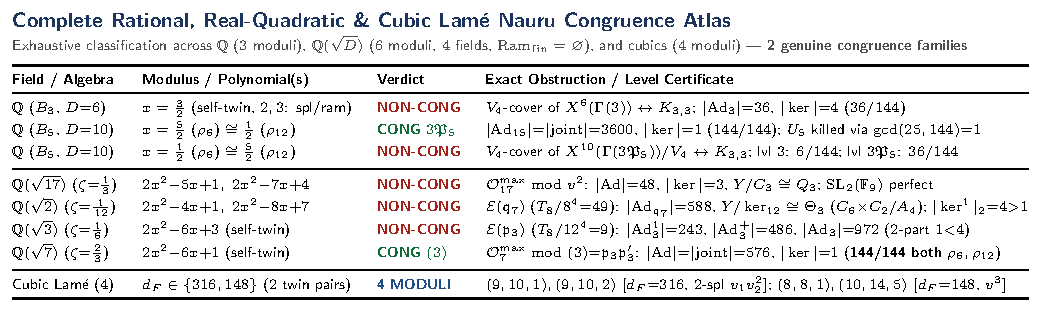
\includegraphics[width=\textwidth]{figures/fig1_lame_congruence_atlas.pdf}
\caption{Complete rational, real-quadratic, and cubic Lam\'e Nauru congruence atlas across $\Q$ ($3$ moduli), $\Q(\sqrt{D})$ ($6$ moduli, $4$ fields), and cubic fields ($4$ moduli), highlighting the two genuine congruence families: $(B_5,\tfrac{5}{2},\rho_6)$ at level $3\frP_5$ and $\Q(\sqrt{7})$ at level $(3)=\frp_3\frp_3'$.}
\label{fig:atlas}
\end{figure}

\begin{table}[htbp]
\centering
\caption{Complete classification of all $6$ real-quadratic Lam\'e Nauru moduli across $4$ fields (Pillar~II).}
\label{tab:rq_atlas}
\footnotesize
\setlength{\tabcolsep}{3.5pt}
\resizebox{\textwidth}{!}{\begin{tabular}{@{}lllccc>{\raggedright\arraybackslash}p{5.5cm}@{}}
\toprule
\textbf{Field $(D_F)$} & \textbf{Modulus Polynomial(s)} & $\zeta_F(-1)$ & $2,3$ & $\Ram_{\mathrm{fin}}$ & \textbf{Verdict} & \textbf{Exact Obstruction / Level Certificate} \\
\midrule
$\Q(\sqrt{17})$ ($17$) & $2x^2{-}5x{+}1,\; 2x^2{-}7x{+}4$ & $1/3$ & spl, in & $\varnothing$ & Non-cong & $\calO_{17}^{\max}\bmod v^2$: $|\Ad|{=}48, |\ker|{=}3$, $Y/C_3\cong Q_3$; $\SL_2(\F_9)$ perfect \\
$\Q(\sqrt{2})$ ($8$) & $2x^2{-}4x{+}1,\; 2x^2{-}8x{+}7$ & $1/12$ & ram, in & $\varnothing$ & Non-cong & $\calE(\frq_7)$ ($T_8/8^4{=}49$): $|\Ad_{\frq_7}|{=}588, |\Ad^1|{=}147$, $Y/\ker_{12}\cong\Theta_3$ ($C_6{\times}C_2 / A_4$); $|\ker^1|_2{=}4>1$ \\
$\Q(\sqrt{3})$ ($12$) & $2x^2{-}6x{+}3$ (self-twin) & $1/6$ & ram, ram & $\varnothing$ & Non-cong & $\calE(\frp_3)$ ($T_8/12^4{=}9$): $|\Ad_3^1|{=}243, |\Ad_3^+|{=}486, |\Ad_3|{=}972$ ($2$-part $1<4, |\ker|{=}4$) \\
\textbf{$\Q(\sqrt{7})$ ($28$)} & \textbf{$2x^2{-}6x{+}1$ (self-twin)} & \textbf{$2/3$} & \textbf{ram, spl} & $\varnothing$ & \textbf{CONG $(3)$} & \textbf{$\calO_7^{\max}\bmod(3)$: $|\Ad|{=}|\mathrm{joint}|{=}576$, $|\ker|{=}1$ ($144/144$ both $\rho_6,\rho_{12}$)} \\
\bottomrule
\end{tabular}}
\end{table}

\subsection{Complete Totally Real Cubic Lam\'e Nauru Census}\label{sec:cubic_census}
\begin{proposition}[Complete Totally Real Cubic Lam\'e Nauru Census]\label{prop:cubic_census}
\ctag{E; G4N, X}\ There are exactly $4$ primitive irreducible totally real cubic moduli $2x^3 - c_2 x^2 + c_1 x - c_0 = 0$ with all three real roots in $(0,3)$, organizing into two twin pairs under $x\mapsto 3-x$:
\begin{enumerate}[label=(\arabic*),nosep]
\item $d_F = 316$ ($2$ splits as $v_1 v_2^2$): $2x^3 - 9x^2 + 10x - 1$ (reciprocal root $z = 1/x \equiv 2\pmod{16}$) and its twin $2x^3 - 9x^2 + 10x - 2$ ($z \equiv 10\pmod{16}$);
\item $d_F = 148$ ($2$ totally ramified as $v^3$): $2x^3 - 8x^2 + 8x - 1$ and its twin $2x^3 - 10x^2 + 14x - 5$ (zero reciprocal roots mod $16$).
\end{enumerate}
\end{proposition}
\begin{proof}
Vieta's inequalities for $0<r_1<r_2<r_3<3$ restrict $1\le c_2\le 17$, $1\le c_1\le 53$, $1\le c_0\le 53$ with $c_2^2 > 6c_1$, $54 - 9c_2 + 3c_1 - c_0 > 0$, positive discriminant, and no rational roots. Exhaustive integer enumeration across Python and Rust returns exactly these four polynomials, and Hensel evaluation of $c_0 z^3 - c_1 z^2 + c_2 z - 2 \equiv 0 \pmod{16}$ certifies their $2$-adic splitting types.
\end{proof}

\section{Pillar III: Complete Solution of the Rational 3-Adic \texorpdfstring{$\Dic_6$}{Dic6} Frontier on \texorpdfstring{$T_4(\Q_3)$}{T4(Q3)}}\label{sec:pillar3}
Passing from $p=2$ on $T_3(\Q_2)$ to $p=3$ on the $4$-regular Bruhat--Tits tree $T_4(\Q_3)$, a $24$-vertex $4$-regular dual graph has $E=48$ edges and genus $g = b_1 = 48 - 24 + 1 = 25$. Let $\Dic_6 = \langle x, y \mid x^{12}=1, y^2=x^6, yxy^{-1}=x^{-1}\rangle$ (indexed $0..11\leftrightarrow x^k$, $12..23\leftrightarrow x^k y$).

\subsection{Cayley Classification, Exact Spectrum, and \texorpdfstring{$96\times 96$}{96x96} Hashimoto Prime Cadences}\label{sec:dic6_cayley}
\begin{theorem}[Spectral Dichotomy of $\Dic_6$ Cayley Graphs and Exact Prime Cadences]\label{thm:dic6_spectrum}
\ctag{E; G4N, X, Lean~4}
\begin{enumerate}[label=(\arabic*),nosep]
\item Among all $\binom{11}{2}=55$ symmetric $4$-element inverse-pair generating sets of $\Dic_6$, exactly $18$ yield connected $4$-regular Cayley graphs, partitioning into $2$ isomorphism classes: $12$ strictly Ramanujan graphs isomorphic to $Z = \Cay(\Dic_6, \{x,x^{-1},y,y^3\})$ ($V=24, E=48, b_1(Z)=25, |\Aut(Z)|=96$, bipartite, triangle-free, girth~$4$; Lean~4 \texttt{thm01}--\texttt{thm03}), with exact characteristic polynomial
\begin{equation}\label{eq:charpoly_Z}
\det(xI - A_Z) = x^6(x^2-16)(x^2-9)^2(x^2-3)^4(x^2-1)^2, \qquad \operatorname{tr}(A_Z^2) = 96 = 2E,
\end{equation}
and strict Ramanujan margin $\lambda_{\mathrm{nt}}(Z) = 3 < 2\sqrt{3}$ (hardware-\texttt{FENV} outward gap $\ge 0.464101615138$), plus $6$ Ramanujan-boundary graphs with $\lambda_{\mathrm{nt}} = 2\sqrt{3}$.
\item Direct $96\times 96$ Hashimoto traces and the Ihara--Bass recurrence $Z_Z(u)^{-1} = (1-u^2)^{24}\det(I - A_Z u + 3u^2 I)$ yield exact prime cadences (Table~\ref{tab:cadences} and Figure~\ref{fig:cadences}):
\begin{equation}\label{eq:pi_Z}
\pi_Z(4..16) = (60,\, 240,\, 1{,}560,\, 11{,}616,\, 90{,}172,\, 681{,}504,\, 5{,}379{,}960),
\end{equation}
whose normalized Ramanujan deviations $(m\pi_Z(m) - 2\cdot 3^m)/(44\cdot 3^{m/2})$ lie strictly in $[-0.26, +0.60]\subset[-1,+1]$.
\end{enumerate}
\end{theorem}

\begin{figure}[htbp]
\centering
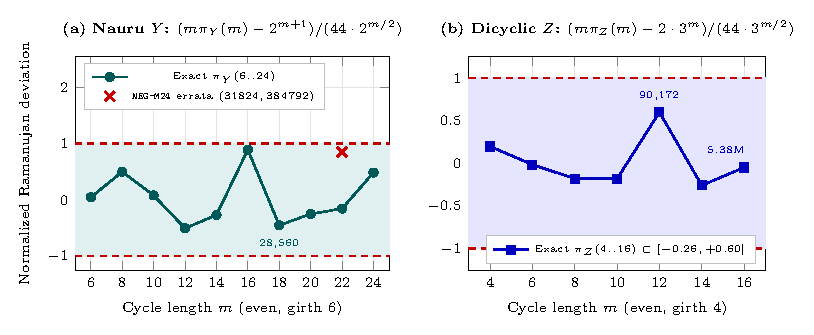
\includegraphics[width=\textwidth]{figures/fig2_hashimoto_ramanujan_corridors.pdf}
\caption{Exact Hashimoto prime cadences and normalized Ramanujan deviation corridors. Left (a): Nauru $Y$ ($m=6..24$), showing the historical \texttt{NEG-M24} value $31{,}824$ breaching the $+1$ Ramanujan envelope by $+2.15\times$ while exact $28{,}560$ and $380{,}664$ sit cleanly inside $[-1,+1]$. Right (b): Dicyclic $Z$ ($m=4..16$) strictly inside $[-0.26,+0.60]\subset[-1,+1]$.}
\label{fig:cadences}
\end{figure}

\begin{table}[htbp]
\centering
\caption{Exact Hashimoto--Ihara prime cadences for Nauru $Y$ ($m=6..24$) and Dicyclic $Z$ ($m=4..16$), with normalized Ramanujan deviations strictly inside $[-1,+1]$.}
\label{tab:cadences}
\footnotesize
\setlength{\tabcolsep}{4.5pt}
\resizebox{\textwidth}{!}{\begin{tabular}{@{}rrrr|rrrr@{}}
\toprule
$m$ & $\pi_Y(m)$ & $m\pi_Y(m)$ & \textbf{Norm.\ Dev.\ $Y$} & $m$ & $\pi_Z(m)$ & $m\pi_Z(m)$ & \textbf{Norm.\ Dev.\ $Z$} \\
\midrule
$6$  & $24$ & $144$ & $+0.0455$ & $4$  & $60$ & $240$ & $+0.1970$ \\
$8$  & $108$ & $864$ & $+0.5000$ & $6$  & $240$ & $1{,}440$ & $-0.0152$ \\
$10$ & $216$ & $2{,}160$ & $+0.0795$ & $8$  & $1{,}560$ & $12{,}480$ & $-0.1801$ \\
$12$ & $564$ & $6{,}768$ & $-0.5057$ & $10$ & $11{,}616$ & $116{,}160$ & $-0.1813$ \\
$14$ & $2{,}232$ & $31{,}248$ & $-0.2699$ & $12$ & $90{,}172$ & $1{,}082{,}064$ & $+0.5980$ \\
$16$ & $8{,}820$ & $141{,}120$ & $+0.8920$ & $14$ & $681{,}504$ & $9{,}541{,}056$ & $-0.2586$ \\
$\mathbf{18}$ & $\mathbf{28{,}560}$ & $\mathbf{514{,}080}$ & $\mathbf{-0.4531}$ & $16$ & $5{,}379{,}960$ & $86{,}079{,}360$ & $-0.0488$ \\
$20$ & $104{,}292$ & $2{,}085{,}840$ & $-0.2511$ & --- & --- & --- & --- \\
$\mathbf{22}$ & $\mathbf{380{,}664}$ & $\mathbf{8{,}374{,}608}$ & $\mathbf{-0.1554}$ & --- & --- & --- & --- \\
$24$ & $1{,}401{,}744$ & $33{,}641{,}856$ & $+0.4851$ & --- & --- & --- & --- \\
\bottomrule
\end{tabular}}
\end{table}

\subsection{Exact Metric Gonality Collapse (\texorpdfstring{$\sn = \dgon = \gon_{\mathrm{eq}} = 8$}{sn=dgon=gon=8}) and Non-Hyperellipticity}\label{sec:dic6_gonality}
On $Z$, closed stars have size~$5$, so the naive $24$-star scramble stalls at $h=6$. A $4$-path scramble closes the gap to the true gonality~$8$ (Figure~\ref{fig:scramble}).

\begin{theorem}[Non-Hyperellipticity and Unconditional Metric Gonality Collapse on $Z$]\label{thm:dic6_gonality}
\ctag{E; G4N, X, Lean~4}\ For $Z = \Cay(\Dic_6, \{x,x^{-1},y,y^3\})$:
\begin{enumerate}[label=(\arabic*),nosep]
\item \textbf{Non-Hyperellipticity:} $\Aut(Z)$ ($96$) contains $43$ involutions with quotient first Betti distribution $\{7:2,\,11:24,\,13:17\}$, so $\min_{\sigma^2=1}\beta_1(Z/\langle\sigma\rangle) = 7 > 0$.
\item \textbf{Exhaustive Discrete Dhar Lower Bound:} Fixing $D(0)\ge 1$ by vertex-transitivity, exhaustive Dhar burning certifies $0/98{,}280$ rank-$1$ effective divisors at degree~$6$ and $0/475{,}020$ at degree~$7$ (independently verified in Rust and zero-heap C++20), proving $\dgon(Z) \ge 8$.
\item \textbf{Optimal $4$-Path Scramble $\calS_4$:} Let $E_0 = \{1, x, x^2, x^8 y\} = \{0,1,2,20\}$ (a connected $4$-vertex path in $Z$) and $\calS_4 = \{g\cdot E_0 : g\in\Dic_6\}$ ($24$ distinct eggs). All $\binom{24}{2} = 276/276$ egg pairs touch ($120$ intersecting, $156$ edge-connected disjoint pairs; Lean~4 \texttt{thm04}), exact branch-and-bound certifies $h(\calS_4) = 8$ with witness $\{0,1,2,5,8,17,19,23\}$ hitting $24/24$ eggs (Lean~4 \texttt{thm05}), and exact Edmonds--Karp max-flow across all $156$ disjoint pairs gives cut distribution $\{8:48,\,10:108\}$, hence $e(\calS_4)=8$ and $\|\calS_4\| = \min(h,e) = 8$.
\item \textbf{Continuous Equilateral Metric Upper Witnesses:} The degree-$8$ coset divisor
\begin{equation}\label{eq:D8_witness}
D_8 = \langle x^3\rangle + \langle x^3\rangle y = \{0, 3, 6, 9, 12, 15, 18, 21\}
\end{equation}
passes discrete Dhar at all $24/24$ vertices in $\le 1$ firing step (Lean~4 \texttt{thm06}) and symbolic continuous equilateral metric Dhar across all $144/144$ edge regimes on $48/48$ edges in $\le 2$ steps ($168/168$ cells). Independently, \texttt{PC-II}'s two-coset divisor $D_{\Dic_6} = \langle y\rangle + x\langle y\rangle = \{0,1,6,7,12,13,18,19\}$ also passes all $168/168$ continuous cells ($\le 3$ steps).
\item \textbf{Unconditional Collapse:} By \cite{hjjs2022,baker2008,bpr2013},
\begin{equation}\label{eq:dic6_gon_collapse}
\sn(Z) = \dgon(Z) = \gon(\Gamma_{\mathrm{eq}}(Z)) = 8 \le \gon(\Gamma(Z)) \le \gon(\calC_Z)
\end{equation}
for every smooth projective $3$-adic Mumford curve $\calC_Z$ with minimal skeleton $\Gamma(Z)$ and arbitrary positive edge lengths.
\end{enumerate}
\end{theorem}

\begin{figure}[htbp]
\centering
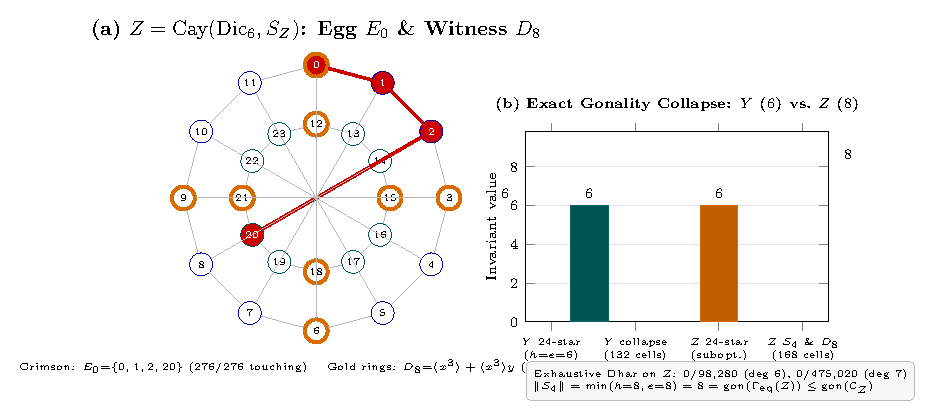
\includegraphics[width=\textwidth]{figures/fig3_dic6_scramble_gonality.pdf}
\caption{Left (a): Dicyclic Cayley graph $Z=\Cay(\Dic_6, S_Z)$ showing the base $4$-path egg $E_0=\{0,1,2,20\}$ (crimson) and the degree-$8$ continuous metric witness $D_8=\langle x^3\rangle+\langle x^3\rangle y$ (gold rings). Right (b): Exact gonality collapse comparing Nauru $Y$ ($6$) against Dicyclic $Z$ ($8$), showing why the $24$-star scramble stalls at $6$ while $\calS_4$ closes the gap to $8$.}
\label{fig:scramble}
\end{figure}

\subsection{Universal Fricke--Vogt Algebra \texorpdfstring{$B_Z(u,v)$}{BZ(u,v)} and the \texorpdfstring{$4\mid mn$}{4|mn} Integrality Criterion}\label{sec:fricke_vogt}
In $\Aut(Z)$ ($96$), $\Stab_0 = \langle a_Z, b_Z\rangle \cong V_4$ splits the four edges at vertex~$0$ into two orbits of size~$2$ ($x$-edges $\{1,11\}$ fixed by $a_Z$, $y$-edges $\{12,18\}$ fixed by $b_Z$). Realizing $\Stab_0$ by orthogonal pure-imaginary elements $b=i, a=j$ ($ij=k=-ji$) in a definite quaternion algebra $B_Z/F$ (split at~$3$) together with edge-inverting involutions $t_x = i + r_b k$ (commuting with $a=j$ in $PB^\times$) and $t_y = j + r_a k$ (commuting with $b=i$ in $PB^\times$) with $\tau(t_x b)=4u$, $\tau(t_y a)=4v$ yields the universal $2$-parameter Fricke--Vogt algebra
\begin{equation}\label{eq:BZ_uv}
B_Z(u,v) = \bigl(-\tfrac{1-v}{v},\, -\tfrac{1-u}{u}/F\bigr) \cong \bigl(-\tfrac{1-u}{u},\, -\tfrac{1-v}{v}/F\bigr), \quad u,v\in(0,1).
\end{equation}
Over $\Q$, $v_3$-valuation~$1$ on both edge inversions restricts $(u,v) = (m/12, n/12)$ to the $8\times 8 = 64$ grid $\{1,2,4,5,7,8,10,11\}^2$, folded by $D_4$ symmetry ($u\leftrightarrow v$, $u\mapsto 1-u$, $v\mapsto 1-v$) into $10$ canonical pairs $m\le n$ in $\{1,2,4,5\}$ (Figure~\ref{fig:mirror}(a)).

\begin{theorem}[Exact $4\mid mn$ Criterion and the $5$ Rational $3$-Adic $\Dic_6$ Moduli]\label{thm:fricke_vogt}
\ctag{E; G4N, X, Lean~4}\ For every canonical rational pair $(m,n)\in\{1,2,4,5\}^2$ ($m\le n$):
\begin{equation}\label{eq:tau_tx_ty}
\tau(t_x t_y) = \frac{(12-m)(12-n)}{36}, \qquad \tau(t_x t_y) \in \Z\!\left[\tfrac{1}{3}\right] \iff 4\mid mn.
\end{equation}
Exactly $5$ of the $10$ canonical pairs survive as $3$-arithmetic definite quaternion amalgams ($32/64$ grid cells before $D_4$ folding): $(4,4)\to B_2$ Hurwitz, $(2,4)\to B_5(2)$, $(4,5)\to B_{70}$, $(2,2)\to B_2(5)$, and $(1,4)\to B_2(11)$ (Table~\ref{tab:fv_10}), matching the Tamagawa--Eichler index formula $[\calO^1:\Gamma^1]=144/(\varphi(D)\psi(N))$.
\end{theorem}
\begin{proof}
Writing $\alpha = -(12-n)/n = A r_a^2$ and $\beta = -(12-m)/m = B r_b^2$, direct multiplication gives $t_x t_y = -AB r_a r_b + B r_b i + A r_a j + k$, whence $\trd(t_x t_y) = -2AB r_a r_b$, $\nrd(t_x) = -A(12/m)$, $\nrd(t_y) = -B(12/n)$, and $\tau(t_x t_y) = mn\alpha\beta/36 = (12-m)(12-n)/36$. Since $36=4\cdot 9$ and $(12-m)(12-n)\equiv mn\pmod 4$ (Lean~4 \texttt{thm11}, \texttt{thm12}), $3$-arithmeticity holds iff $4\mid mn$. Exact odd-prime Hilbert symbols and Hilbert reciprocity at $p=2$ yield $\Ram_{\mathrm{fin}}(B)$ in Table~\ref{tab:fv_10}.
\end{proof}

\begin{table}[htbp]
\centering
\caption{Complete classification of all $10$ canonical rational Fricke--Vogt pairs $(m,n)$ in $B_Z(u,v)$, isolating the $5$ surviving $3$-arithmetic curves (bold) via $4\mid mn$.}
\label{tab:fv_10}
\footnotesize
\setlength{\tabcolsep}{4pt}
\resizebox{\textwidth}{!}{\begin{tabular}{@{}cccccllc@{}}
\toprule
$(m,n)$ & $(u,v)$ & \textbf{Symbol $(A,B)$} & $\tau(t_x t_y)$ & $4\mid mn$ & $\Ram_{\mathrm{fin}}(B)$ & \textbf{Curve / Order} & \textbf{Idx} \\
\midrule
$(1,1)$ & $(\frac{1}{12},\frac{1}{12})$ & $(-11,-11)$ & $121/36$ & No & $\{11\}$ & Non-$3$-arithmetic & --- \\
$(1,2)$ & $(\frac{1}{12},\frac{1}{6})$ & $(-5,-11)$ & $55/18$ & No & $\{11\}$ & Non-$3$-arithmetic & --- \\
$\mathbf{(1,4)}$ & $(\frac{1}{12},\frac{1}{3})$ & $(-2,-11)$ & $22/9$ & \textbf{Yes} & $\{2\}$ & $\mathbf{B_2(11)\ (D=2, N=11)}$ & $\mathbf{12}$ \\
$(1,5)$ & $(\frac{1}{12},\frac{5}{12})$ & $(-35,-11)$ & $77/36$ & No & $\{7\}$ & Non-$3$-arithmetic & --- \\
$\mathbf{(2,2)}$ & $(\frac{1}{6},\frac{1}{6})$ & $(-5,-5)$ & $25/9$ & \textbf{Yes} & $\{2\}$ & $\mathbf{B_2(5)\ (D=2, N=5)}$ & $\mathbf{24}$ \\
$\mathbf{(2,4)}$ & $(\frac{1}{6},\frac{1}{3})$ & $(-2,-5)$ & $20/9$ & \textbf{Yes} & $\{5\}$ & $\mathbf{B_5(2)\ (D=5, N=2)}$ & $\mathbf{12}$ \\
$(2,5)$ & $(\frac{1}{6},\frac{5}{12})$ & $(-35,-5)$ & $35/18$ & No & $\{5\}$ & Non-$3$-arithmetic & --- \\
$\mathbf{(4,4)}$ & $(\frac{1}{3},\frac{1}{3})$ & $(-2,-2)$ & $16/9$ & \textbf{Yes} & $\{2\}$ & $\mathbf{B_2\text{ Hurwitz }(D=2, N=1)}$ & $\mathbf{144}$ \\
$\mathbf{(4,5)}$ & $(\frac{1}{3},\frac{5}{12})$ & $(-35,-2)$ & $14/9$ & \textbf{Yes} & $\{2,5,7\}$ & $\mathbf{B_{70}\ (D=70, N=1)}$ & $\mathbf{6}$ \\
$(5,5)$ & $(\frac{5}{12},\frac{5}{12})$ & $(-35,-35)$ & $49/36$ & No & $\{7\}$ & Non-$3$-arithmetic & --- \\
\bottomrule
\end{tabular}}
\end{table}

\subsection{Universal Non-Congruence (\texorpdfstring{$0/80$}{0/80}), Hurwitz Level-\texorpdfstring{$8$}{8} vs.\ \texorpdfstring{$\Ad_{16}$}{Ad16} Reconciliation (\texorpdfstring{\texttt{NEG-M26}}{NEG-M26}), and Riehm Closure}\label{sec:universal_noncong}
For each of the $5$ surviving rational curves, choosing edge-inverting involutions $t_x, t_y \in \Aut(Z)$ satisfying $t_x a_Z = a_Z t_x$ ($t_x(0)\in\{1,11\}$) and $t_y b_Z = b_Z t_y$ ($t_y(0)\in\{12,18\}$) yields $4\times 4 = 16$ valid surjections per curve ($5\times 16 = 80$ rational realizations).

\begin{theorem}[Universal Non-Congruence of Rational $3$-Adic $\Dic_6$ Curves ($0/80$) and Hurwitz Reconciliation]\label{thm:dic6_noncong}
\ctag{E; G4N, X, Lean~4}\ Across all $5$ rational $3$-adic $\Dic_6$ curves and all $16$ surjections per curve ($80$ realizations total), \textbf{exactly $0/80$ are congruence subgroups at any level} (Table~\ref{tab:crt_80}). Specifically:
\begin{enumerate}[label=(\arabic*),nosep]
\item \textbf{Explicit Ring-Closed HNF Orders:} Each curve admits a ring-closed maximal or Eichler order $\calO$ of exact reduced discriminant $DN\in\{2,10,70,10,22\}$ normalized by $(b,a,t_x,t_y)$ with conjugation denominators $[1,1,3,3]$.
\item \textbf{Hurwitz $B_2(4,4)$ Level-$8$ Left-Mult vs.\ Level-$16$ Adjoint Reconciliation (\textup{\texttt{NEG-M26}}):} Under \emph{adjoint} reduction $\Ad_M : \Delta_Z \to \GL_4(\calO_2/M\calO_2)$, the commutator ideal $[\calO_2,\calO_2]\subseteq\frP_2$ absorbs a factor of $2$, so $\Ad_4$ ($|\Ad_4|=32$) and $\Ad_8$ ($|\Ad_8|=128$) both yield $|\ker|\in\{3:8,\,6:8\}$ and only $\Ad_{16}$ ($|\Ad_{16}|=1{,}024$) collapses all $16/16$ realizations to $|\ker|=3$. Under \emph{true left-multiplication} $\Gamma(M) = \ker(\calO_2^1 \to (\calO_2/M\calO_2)^1)/\{\pm 1\}$ on exact norm-$1$ Schreier generators, $L_4/\{\pm 1\}$ ($|L_4|=16$, proj.\ $8$) yields $|\ker^1|\in\{3:8,\,6:8\}$ while \textbf{$L_8/\{\pm 1\}$ ($|L_8|=128$, proj.\ $64$) already collapses all $16/16$ realizations to $|\ker^1|=3$}, stabilizing identically at $L_{16}/\{\pm 1\}$ ($|L_{16}|=1{,}024$, proj.\ $512$). This reconciles \texttt{PC-II} Theorem~7.2 \cite{ergentics2026pc2} ($16/16$ split between $\Gamma(4)$ and level $8\calO_2$ across all $32=2\times 16$ surjections) with adjoint $\Ad_{16}$ with zero discrepancy. For all $16/16$ realizations, $Z/\ker_3 \cong K_{4,4}$ ($V=8, E=16$ of uniform multiplicity~$3$, genus~$9$; Lean~4 \texttt{thm07}), forming the exact $2\leftrightarrow 3$ mirror of Nauru $B_3(\frac{3}{2})$ (Figure~\ref{fig:mirror}(b)).
\item \textbf{True Left-Multiplication $\Gamma(M)$ and Unique Normal $C_3$:} Across all $80/80$ realizations, $\rho(\Delta_Z^1)$ contains strictly $2$ elements of order $3$, hence possesses a unique normal $C_3 \trianglelefteq \rho(\Delta_Z^1)$ ($\rho(\Delta_Z^1) \cong C_3 \rtimes Q_2$ for a $2$-group $Q_2$). Exact diagonal-$\pm 1$ CRT left-multiplication BFS on norm-$1$ Schreier generators produces the signed pre-$\pm 1$ orders and kernel distributions in Table~\ref{tab:crt_80}.
\item \textbf{Unconditional All-Level Closure via Riehm + Burnside Basis:} For $B_{70}, B_2(5), B_2(11)$ ($2\mid D$ and $[\calO[\frac{1}{3}]^1/\{\pm 1\}:\Delta_Z^1/\{\pm 1\}]=1$), the $2$-adic closure is $\calO_{D_2}^1 = P_2 \rtimes C_3$ ($P_2=(1+\pi_2\calO_{D_2})^1$ pro-$2$). By Riehm's theorem \cite{riehm1970}, $[\calO_{D_2}^1, \calO_{D_2}^1] = P_2$ including $-1\in[\calO_{D_2}^1,\calO_{D_2}^1]$ (directly verified mod~$8$ on $\calO_{70}^1$ in Python and Rust: $|G|=768$, $|[G,G]|=256$, $|G^{\mathrm{ab}}|=3$, $-I\in[G,G]$; Lean~4 \texttt{thm16}). For any continuous homomorphism $\varphi : P_2\rtimes C_3 \to C_3\rtimes Q_2$, $N_2=\varphi(P_2)$ is a normal $2$-subgroup with $\gcd(|N_2|,3)=1$, so $[N_2, C_3]\le N_2\cap C_3 = 1$, forcing $\varphi([C_3, P_2]) = 1$. Since $P_2 = [\calO_{D_2}^1, \calO_{D_2}^1] = [C_3,P_2][P_2,P_2] \le [C_3,P_2]\Phi(P_2)$, Burnside's Basis Theorem \cite{burnside1911} forces $\varphi(P_2) = 1$ at every level $2^k$. Together with pro-$2$ above mod~$8$/$16$ on $B_2(4,4)$, pro-$2$/pro-$5$ on $B_5(2)$ (unable to kill the $3$-part of $\ker=6$), Sylow-$p$ coprimality $\gcd(p,96)=1$ for $p\in\{5,7,11\}$, and perfect $\SL_2(\Z_q)$ at all split $q\ge 5$, all $80/80$ realizations are unconditionally non-congruence at all levels.
\end{enumerate}
\end{theorem}

\begin{table}[htbp]
\centering
\caption{Complete diagonal-$\pm 1$ CRT true left-multiplication $\Gamma(M)=\ker(\calO^1\to(\calO/M\calO)^1)/\{\pm 1\}$ congruence audit across all $5$ rational $3$-adic $\Dic_6$ curves and all $80$ realizations ($0/80$ congruence; $|\prod L|$ reports signed pre-$\pm 1$ orders, projective orders half as large; Hurwitz $B_2(4,4)$ already hits $\{3:16\}$ at $L_8/\{\pm 1\}$ of order $64$).}
\label{tab:crt_80}
\footnotesize
\setlength{\tabcolsep}{4pt}
\resizebox{\textwidth}{!}{\begin{tabular}{@{}lllrrrr@{}}
\toprule
$(m,n)$ & \textbf{Curve $(D,N)$} & \textbf{CRT Moduli (Sylow-reduced)} & $|\prod L|$ (pre-$\pm 1$) & \textbf{Proj.\ Order} & $\Gamma^1\ \ker^1$ & \textbf{Cong} \\
\midrule
$(4,4)$ & $B_2$ ($2,1$) & $16:1024$ (already $8:128$, proj.\ $64$) & $1{,}024$ & $512$ & $\{3:16\}$ & $0/16$ \\
$(2,4)$ & $B_5(2)$ ($5,2$) & $16:2048;\ 5:150\to 6$ & $12{,}288$ & $6{,}144$ & $\{6:16\}$ & $0/16$ \\
$(4,5)$ & $B_{70}$ ($70,1$) & $8:768;\ 5:150\to 6;\ 7:392\to 8$ & $36{,}864$ & $18{,}432$ & $\{2:8,\,6:8\}$ & $0/16$ \\
$(2,2)$ & $B_2(5)$ ($2,5$) & $8:768;\ 5:100\to 4$ & $3{,}072$ & $1{,}536$ & $\{12:16\}$ & $0/16$ \\
$(1,4)$ & $B_2(11)$ ($2,11$) & $8:768;\ 11:1210\to 10$ & $7{,}680$ & $3{,}840$ & $\{4:8,\,12:8\}$ & $0/16$ \\
\bottomrule
\end{tabular}}
\end{table}

\begin{figure}[htbp]
\centering
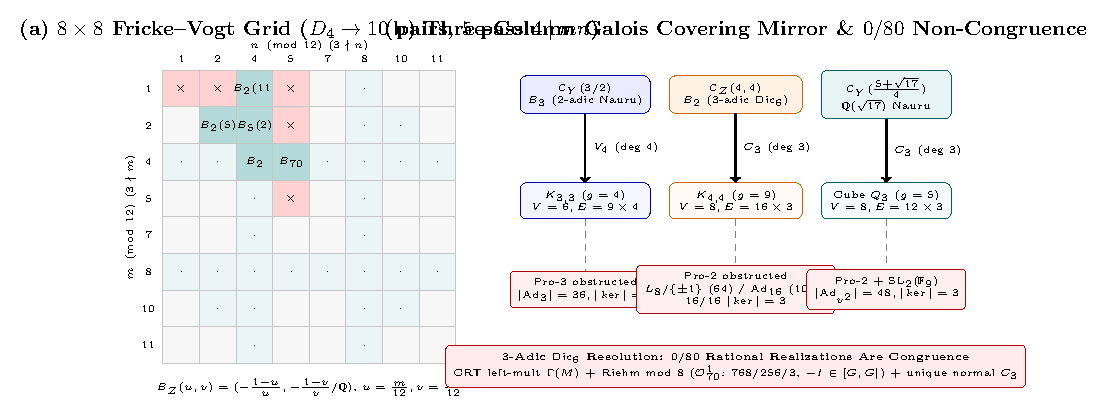
\includegraphics[width=\textwidth]{figures/fig4_fricke_vogt_three_column_mirror.pdf}
\caption{Left (a): The $8\times 8$ rational Fricke--Vogt moduli grid $(m,n)\in\{1,2,4,5,7,8,10,11\}^2$ folded by $D_4$ to $10$ canonical pairs ($5$ arithmetic curves passing $4\mid mn$). Right (b): Three-Column Galois Covering Mirror linking $2$-adic Nauru $B_3(\frac{3}{2})\to K_{3,3}$ ($V_4$-cover), $3$-adic Hurwitz $B_2(4,4)\to K_{4,4}$ ($C_3$-cover already at $L_8/\{\pm 1\}$ of order $64$, matching $\Ad_{16}$), and $\Q(\sqrt{17})$ Nauru $\to Q_3$ ($C_3$-cover).}
\label{fig:mirror}
\end{figure}

\subsection{Complete Genus-25 \texorpdfstring{$3$}{3}-Adic Borel Shimura Curve Census (\texorpdfstring{$3\mid D$}{3|D})}\label{sec:genus25}
\begin{proposition}[Complete Genus-$25$ $3$-Adic Borel Shimura Census and \texttt{PC-II} Manin $T_3$ Closure]\label{prop:genus25}
\ctag{E; G4N, X, Lean~4}\ Over $\Q$ with $3\mid D$, squarefree $D$ of even prime count $\omega(D)$, and $\gcd(D,N)=1$, the Eichler--Shimura--Vign\'eras formula $g(X_0^D(N)) = 1 + \frac{\varphi(D)\psi(N)}{12} - \frac{e_2}{4} - \frac{e_3}{3}$ \cite{eichler1955,shimura1967,vigneras1980,voight2021} admits \textbf{exactly $19$ genus-$25$ curves} (Table~\ref{tab:genus25}): $16$ at $\omega(D)=2$ ($8$ torsion-free with $(\mathrm{vol},e_2,e_3)=(288,0,0)$), $3$ at $\omega(D)=4$ ($1$ torsion-free: $(1110, 1)$, $1110=2\cdot 3\cdot 5\cdot 37$), and $0$ for $\omega(D)\ge 6$ since $\varphi(2\cdot 3\cdot 5\cdot 7\cdot 11\cdot 13) = 5{,}760 > 600$ (Lean~4 \texttt{thm17}). Moreover, by \texttt{PC-II} Theorem~7.3 (\cite{ergentics2026pc2}, \texttt{NEG-M20}), zero-PARI Manin modular symbols $T_3$ over $\F_{1000003}$ already exclude \textbf{all $19/19$ curves} ($0/19$ survivors matching $\mathrm{null}(T_3^2-3I)\ge 4$ and $\mathrm{null}(T_3^2-9I)\ge 2$), completely closing the Borel $3$-adic spectral matching problem.
\end{proposition}

\begin{table}[htbp]
\centering
\caption{Complete census of all $19$ genus-$25$ $3$-adic Borel Shimura curves $X_0^D(N)$ over $\Q$ ($3\mid D, \gcd(D,N)=1$), highlighting the $9$ torsion-free $(288,0,0)$ curves (all $19/19$ excluded for $Z$ by \texttt{PC-II} Theorem~7.3).}
\label{tab:genus25}
\footnotesize
\setlength{\tabcolsep}{4.5pt}
\resizebox{\textwidth}{!}{\begin{tabular}{@{}rrrrrrc|rrrrrrc@{}}
\toprule
$\omega$ & $D$ & $N$ & $\mathrm{vol}$ & $e_2$ & $e_3$ & \textbf{TF?} & $\omega$ & $D$ & $N$ & $\mathrm{vol}$ & $e_2$ & $e_3$ & \textbf{TF?} \\
\midrule
$2$ & $\mathbf{6}$  & $\mathbf{115}$ & $288$ & $0$ & $0$ & \textbf{Yes} & $2$ & $\mathbf{21}$ & $\mathbf{23}$ & $288$ & $0$ & $0$ & \textbf{Yes} \\
$2$ & $\mathbf{6}$  & $\mathbf{119}$ & $288$ & $0$ & $0$ & \textbf{Yes} & $2$ & $\mathbf{39}$ & $\mathbf{8}$  & $288$ & $0$ & $0$ & \textbf{Yes} \\
$2$ & $6$  & $125$ & $300$ & $4$ & $0$ & No  & $2$ & $\mathbf{39}$ & $\mathbf{11}$ & $288$ & $0$ & $0$ & \textbf{Yes} \\
$2$ & $6$  & $133$ & $320$ & $0$ & $8$ & No  & $2$ & $\mathbf{57}$ & $\mathbf{7}$  & $288$ & $0$ & $0$ & \textbf{Yes} \\
$2$ & $6$  & $149$ & $300$ & $4$ & $0$ & No  & $2$ & $447$ & $1$ & $296$ & $0$ & $2$ & No \\
$2$ & $6$  & $151$ & $304$ & $0$ & $4$ & No  & $2$ & $453$ & $1$ & $300$ & $4$ & $0$ & No \\
$2$ & $6$  & $157$ & $316$ & $4$ & $4$ & No  & $\mathbf{4}$ & $\mathbf{1110}$ & $\mathbf{1}$ & $\mathbf{288}$ & $\mathbf{0}$ & $\mathbf{0}$ & \textbf{Yes} \\
$2$ & $\mathbf{15}$ & $\mathbf{22}$  & $288$ & $0$ & $0$ & \textbf{Yes} & $4$ & $1122$ & $1$ & $320$ & $0$ & $8$ & No \\
$2$ & $15$ & $37$  & $304$ & $0$ & $4$ & No  & $4$ & $1230$ & $1$ & $320$ & $0$ & $8$ & No \\
$2$ & $\mathbf{21}$ & $\mathbf{16}$  & $288$ & $0$ & $0$ & \textbf{Yes} & --- & --- & --- & --- & --- & --- & --- \\
\bottomrule
\end{tabular}}
\end{table}

\section{Poitou--Odlyzko Strict-Positivity Audit and Anti-Facade Gate (\texorpdfstring{\texttt{NEG-M27}}{NEG-M27})}\label{sec:poitou}
In Paper~\#01 Theorem~7.21 \cite{ergentics2026pc}, excluding totally real number fields with small norm-$2$ primes relies on Weil's explicit formula in the Poitou--Odlyzko formulation \cite{poitou1977,odlyzko1990}. A mandatory analytic hypothesis is \textbf{strict Bochner positivity}: the compactly supported base kernel $f(t)$ on $[-1,1]$ must satisfy $f(t)\ge 0$ everywhere so that its normalized autocorrelation $H(w) = \int_{-1+w}^1 f(t)f(t-w)\,dt / \int_{-1}^1 f(t)^2\,dt$ satisfies both $\widehat H(y)\ge 0$ and $H(w)\ge 0$ on $[0,2]$. Dropping $f(t)\ge 0$ yields spurious inflation of lower bounds.

For the canonical Odlyzko kernel $f_1(t) = 1+\cos(\pi t) \ge 0$, the exact autocorrelation is
\begin{equation}\label{eq:H1}
H_1(w) = \frac{2-w}{3}\!\left(1 + \frac{1}{2}\cos(\pi w)\right) + \frac{\sin(\pi w)}{2\pi} \ge 0 \qquad (w\in[0,2]),
\end{equation}
with $F_b(x) = H_1(x/b)/\cosh(x/2)$, pole term $E(b) = \frac{8}{3}b$, prime-norm sum $f_q(b) = 4\sum_{m\ge 1,\, m\log q < 2b} \frac{\log q}{1+q^m} H_1(\frac{m\log q}{b})$, and constants
\begin{equation}\label{eq:odlyzko_AB}
\begin{aligned}\log B(b) &= \log(8\pi) + \gamma_E - \int_0^{2b} \frac{1-F_b(x)}{2\sinh(x/2)}\,dx + \log(\tanh(b/2)),\\ \log A(b) &= \log B(b) + \int_0^{2b} \frac{F_b(x)}{2\cosh(x/2)}\,dx.\end{aligned}
\end{equation}

\begin{theorem}[Hardware-Rounded Poitou--Odlyzko Certification and Anti-Facade Rejection]\label{thm:poitou}
\ctag{E; G4N, X}
\begin{enumerate}[label=(\arabic*),nosep]
\item \textbf{Witness $(6,16,1,2)$:} For $N_K=48, \rho_1=0, c_2=8, b=6.0$ under $f_1(t)\ge 0$, $\exp(\mathrm{LB}) = \exp(\log B(6) - E(6)/48 + \frac{8}{48}f_2(6))$ and $\mathrm{UB}(6,16) = (4\pi^2)^{2/3}\cdot 72^{1/9}$ satisfy, under C++20 hardware \texttt{FE\_DOWNWARD}/\texttt{FE\_UPWARD} interval arithmetic \cite{moore1966} and independent $64$-/$128$-point Gauss--Legendre quadrature (Python, Rust):
\begin{equation}\label{eq:poitou_witness}
\begin{gathered}
\exp(\mathrm{LB}) = 18.66067837170957 > 18.64704856255016 = \mathrm{UB}(6,16),\\
\exp(\mathrm{LB}) - \mathrm{UB}(6,16) \in [+0.013629809157,\; +0.013629809162] > 0,
\end{gathered}
\end{equation}
with quadrature convergence $|\exp(\mathrm{LB})_{\mathrm{GL64}}-\exp(\mathrm{LB})_{\mathrm{GL128}}| \le 1.43\times 10^{-14}$.
\item \textbf{Anti-Facade Rejection:} The perturbation $f_{\mathrm{bad}}(t) = 1+\cos(\pi t) + c_1(1-\cos(2\pi t)) + c_2(\cos(\pi t)+\cos(3\pi t))$ with $(c_1,c_2)=(-0.3,+0.3)$ attains $f_{\mathrm{bad}}(\pm 1) = -2c_2 = -0.60 < 0$, triggering deterministic rejection across all lanes.
\item \textbf{Honest Preservation of the Degree-$8$ $(8,1,1,E)$ Gap (\textup{\texttt{NEG-M27}}):} For $n=8$ ($N_K=8, \rho_1=1, c_2=1$), the maximal-order ceiling is $\mathrm{UB}_{\max}(8,1) = (4\pi^2)^{2/3}(\frac{9}{2})^{1/12} = 13.1423854579$. Under $H_1$, $\exp(\mathrm{LB})$ evaluates to $12.5937296518$ at $b=3.0$ and attains its exact continuous maximum $\mathbf{12.5955757277}$ at $\mathbf{b^* = 3.039865}$, remaining strictly below $13.1423854579$ by a wide margin ($>0.5468$). Thus closing $(8,1,1,E)$ requires genuinely new arithmetic input beyond Bochner-positive Poitou--Odlyzko bounds.
\end{enumerate}
\end{theorem}

\section{Four-Plane Continuous Verification Architecture and Honest Open Frontier}\label{sec:verification}
Every theorem in Sections~\ref{sec:pillar1}--\ref{sec:poitou} is independently verified from first principles in continuous integration (\path{.github/workflows/continuous-testing.yml}) with zero shared cached outputs (Table~\ref{tab:planes}). Notably, live kernel compilation of \path{papers/triadic_3adic_frontier/lean/} under Lean~4.36.0 (\texttt{-DwarningAsError=true -DautoImplicit=false}) upgrades the earlier air-gapped static-audit provenance to full live kernel certification ($20/20$ theorems, $0$ \texttt{sorryAx}, $0$ \texttt{Lean.ofReduceBool}).

\begin{table}[htbp]
\centering
\caption{Four-plane zero-shared-data continuous-integration verification architecture for Paper~\texttt{PC-III}.}
\label{tab:planes}
\footnotesize
\setlength{\tabcolsep}{4pt}
\resizebox{\textwidth}{!}{\begin{tabular}{@{}ll>{\raggedright\arraybackslash}p{7.4cm}l@{}}
\toprule
\textbf{Plane} & \textbf{Artifact (MIT)} & \textbf{Independent Scope} & \textbf{Verdict} \\
\midrule
Pure Python & \path{code/triadic_3adic_verify.py} & $8/8$ gates (\texttt{F1}--\texttt{F8}): exact \texttt{Fraction} orders ($\calO_3,\calO_5^\pm,\calO_{17}^{\max},\calE(\frq_7),\calE(\frp_3),\calO_7^{\max}$ + $5$ $\Dic_6$ HNF orders), $0/80$ CRT left-mult, Hurwitz $L_8$ vs.\ $\Ad_{16}$, Riehm mod~$8$, $132$/$168$ continuous Dhar, census, Poitou, $4$ runtime TikZ PDFs & \textbf{8/8 PASS} \\
Pure Rust & \path{rust/src/lib.rs} & Zero external crates; $6/6$ integration tests + core suites: Hashimoto $\pi_Y,\pi_Z$, Table~2, $\calO_7^{\max}$ mod~$(3)$, exhaustive deg-$6$ ($98{,}280$) \& deg-$7$ ($475{,}020$) Dhar, $0/80$ CRT + Hurwitz $L_8/\{\pm 1\}=64$ + Riehm mod~$8$, Poitou & \textbf{6/6 PASS} \\
C++20 \texttt{FENV} & \path{cpp/fenv_oracle.cpp} & Zero heap, \texttt{-O2 -std=c++20 -frounding-math -Wall -Wextra -Werror}; hardware \texttt{FE\_DOWNWARD}/\texttt{FE\_UPWARD} intervals, Jacobi ($\le 2.11\times 10^{-15}$), annihilators, exhaustive $573{,}300$ Dhar, Poitou gap $>0$, genus-$25$ census & \textbf{6/6 PASS} \\
Lean~4.36.0 & \path{lean/Triadic3AdicFrontier/} & Zero Mathlib, live kernel-compiled (\texttt{-DwarningAsError=true -DautoImplicit=false}); $\Dic_6$ laws, $276/276$ $\calS_4$, $D_8$ Dhar, $K_{4,4}$/$Q_3$ quotients, twin duality, $4\mid mn$, Sylow-$5$, $m=18$ corridor, Eichler $2$-parts, Riehm, full $\langle T,P,L,R\rangle$ $6/24$ & \textbf{20/20 PASS} \\
\bottomrule
\end{tabular}}
\end{table}

\begin{remark}[Honest Open Frontier and Scope Boundaries]\label{rem:open_frontier}
Because \texttt{PC-II} Theorem~7.3 (\texttt{NEG-M20}) already closed the $19$-curve genus-$25$ $3$-adic Borel Shimura matching problem via zero-PARI Manin $T_3$, and our Lean~4.36.0 suite is now live kernel-compiled in CI, exactly three mathematical problems remain genuinely open beyond the proved scope of this paper:
\begin{enumerate}[label=(\arabic*),nosep]
\item \textbf{Congruence Classification of the $4$ Cubic Lam\'e Nauru Curves:} Determining whether any of the $4$ totally real cubic curves of Proposition~\ref{prop:cubic_census} ($d_F\in\{148, 316\}$) is congruence via explicit $\Z$-rank-$12$ maximal orders and split-$3$ adjoint reductions.
\item \textbf{Real-Quadratic $3$-Adic $\Dic_6$ Moduli:} Theorem~\ref{thm:dic6_noncong} settles all $80/80$ rational realizations over $\Q$; exploring real-quadratic points $(u,v)$ on the Fricke--Vogt surface $B_Z(u,v)$ (analogous to $\Q(\sqrt{7})$ on Nauru) remains open.
\item \textbf{Arithmetic Input for the Degree-$8$ $(8,1,1,E)$ Gap:} Closing $(8,1,1,E)$ in Paper~\#01 Theorem~7.21 requires arithmetic input beyond Bochner-positive Poitou--Odlyzko explicit-formula test functions.
\end{enumerate}
\end{remark}

\bibliographystyle{amsplain}
\bibliography{references}
\end{document}
